\documentclass[aps,prb,reprint,amsmath,amssymb,longbibliography,floatfix]{revtex4-2}

\usepackage{amsthm,mathtools}
\usepackage{array}
\usepackage{booktabs}
\usepackage{graphicx}
\usepackage{xcolor}
\usepackage{tikz}
\usetikzlibrary{arrows.meta,calc,positioning}
\usepackage{pgfplots}
\pgfplotsset{compat=1.18}
\usepackage{microtype}
\makeatletter
\def\label#1{\@bsphack
  \begingroup
  \UseHookWithArguments{label}{1}{#1}%
  \protected@write\@auxout{}%
    {\string\newlabel{#1}{{\@currentlabel}{\thepage}{\@currentlabelname}%
      {\@currentHref}{\@kernel@reserved@label@data}}}%
  \endgroup
  \@esphack}
\makeatother
\usepackage[hidelinks]{hyperref}
\makeatletter
\let\ltx@label\label
\makeatother
\setlength{\emergencystretch}{2em}

\definecolor{protocolblue}{RGB}{31,78,121}
\definecolor{protocolgray}{RGB}{245,247,249}
\newcommand{\norm}[1]{\left\lVert #1\right\rVert}
\newcommand{\C}{\mathbb{C}}
\newcommand{\R}{\mathbb{R}}
\newtheorem{theorem}{Theorem}
\newtheorem{corollary}[theorem]{Corollary}
\newtheorem{proposition}[theorem]{Proposition}

\begin{document}

\title{Band Equivalence Does Not Determine Hopping Locality:
Exact Rank-Two Geometry and Equal-Accuracy Range Inflation}
\author{Eugene Joseph M. Ragasa}
\email{eugene.ragasa@dlsu.edu.ph}
\affiliation{Department of Physics, De La Salle University, Manila, Philippines}
\date{Working Physical Review B revision --- 16 October 2026}

\begin{abstract}
Band spectra are invariant under momentum-dependent unitary similarity, but hopping
locality is not. We derive the exact adequacy geometry for a rank-two candidate that
shifts the energy centroid and positively rescales the traceless level splitting. The
spectral loss and every matrix loss under one momentum-independent real rotation share a
single diagonal quadratic curvature. Their admissible sets are homothetic ellipses
controlled by a splitting scale $\kappa$ and a normalized correlation $\mu$. For the
smooth family $U_a(q)=R(a\sin2\pi q)$, every member has exactly the same bands, while the
minimum restricted-alignment threshold rises as
$\sqrt{\kappa[1-J_0(2a)^2]}$ and the exact-spectrum joint threshold rises as
$\sqrt{2\kappa[1-J_0(2a)]}$. For a spectrally flat traceless parent, we prove that the
squared irreducible matrix residual equals the total Fourier weight transferred to
nonzero-range hopping blocks. Development calculations verify the flat-parent identity,
extend the mechanism through a dispersive four-state homotopy, and separate cyclic
conversion, interpolation, deliberate truncation, and total spectral error. On the dense integer
cutoff inventory $R_c=0,\ldots,16$, the first sampled passing ranges at the fully
dispersive endpoint are 4 and 10 for the reference and rotated representations,
respectively, at a $10^{-8}E_{\mathrm{ref}}$ sampled band-error target. The complete models remain pointwise unitarily equivalent before
truncation. The result is therefore a quantitative statement about representation
efficiency: band equivalence alone does not determine the finite hopping range required
at fixed accuracy.
\end{abstract}
\maketitle

\paragraph{Scope.}
The threshold continuum, admissible-set geometry, and flat-parent locality identity are
analytic. Direct evaluation of the $J_0(2a)$ laws establishes the flat-parent continuum;
no amplitude interpolant supports those claims. The dispersive and truncation results
are sampled development calculations. Consequently, the non-flat claims apply only at
the declared amplitude nodes, and plotted connections are guides to the eye. The dense
inventory gives exact minimization over each declared integer cutoff
$R_c=0,\ldots,16$ but no claim beyond that cap. Final production controls and an
independently verified retained execution remain future work.

\section{Introduction}

Band energies do not determine a Hamiltonian's matrix representation or hopping
locality. A reduced Hamiltonian may reproduce selected bands while failing to reproduce
the matrix field under a declared identification of retained coordinates. Eigenvalues
are invariant under basis rotation; matrix entries and Fourier hopping blocks are not.
When the generating momentum-dependent unitary is admitted as the state-space
identification, the two fields represent the same abstract operator and their residual
vanishes. This study imposes the stricter identification of one momentum-independent
real rotation. Spectral agreement and restricted-alignment agreement are therefore
distinct requirements.

Rather than beginning with a material-derived reduction in which parent-model,
discretization, disentanglement, gauge-selection, and truncation effects coexist, this
work establishes the first rung of a controlled validation ladder. The fully known
periodic parent isolates representation-induced changes in hopping locality from those
other error sources. Section~\ref{sec:validation-ladder} places this one-dimensional,
rank-two benchmark within the planned progression through higher dimensions,
anisotropy, general lattices, higher-rank gauge classes, and ultimately hidden-target
material reductions.

\section{Background and related work}

Gauge-dependent locality is established in the Wannier literature. Wannier functions
inherit the momentum-dependent gauge freedom of their Bloch manifold, and smooth gauges
produce different real-space shapes and spreads. Localized Wannier bases make
Hamiltonian matrices sparse and enable efficient interpolation and large-scale
calculation~\cite{marzari1997,souza2001,yates2007,marzari2012,marrazzo2024}. Local unitary transformations of
all-bands-flat lattices preserve the complete flat spectrum while changing the hopping
construction~\cite{danieli2021}; compact and maximally localized Wannier functions also
need not coincide~\cite{sathe2024}. Systematic improvement with hopping range has been
studied in a Wannier-based one-dimensional photonic model~\cite{gupta2022}. Explicit
truncation degrades band and response accuracy, and band agreement alone does not
validate wavefunction-dependent observables~\cite{ghosh2025}. These works establish the surrounding gauge, localization, and truncation phenomena.
In particular, the maximally localized Wannier-function (MLWF) decomposition
$\Omega=\Omega_{\mathrm I}+\widetilde\Omega$ separates a projector-dependent contribution
to the Wannier spread from a contribution that varies with the chosen Bloch frame. It is
not a theorem for aligning two represented Hamiltonians. The alignment diagnostic used
here instead minimizes a cross-model matrix loss over a separately declared family of
identification maps. Its value depends on both represented operators, the comparison
weights and normalization, and the allowed alignment family; it is invariant under a
frame change only when that entire comparison contract is transported with the frames.
Supplementary Sec.~S1.6 states this limited covariance result and explains why it is not
the MLWF spread decomposition or a new localization principle.

The present work does not claim those surrounding phenomena or this elementary
alignment covariance individually as new. Instead, it supplies a controlled rank-two
benchmark in which the complete Hamiltonians are
pointwise unitarily equivalent, while their agreement under one momentum-independent
real alignment and their finite-range representation costs remain distinct. Within the
declared affine candidate and global $SO(2)$ alignment families, the spectral and
restricted-operator losses have an exact common-curvature geometry. For the smooth flat
parent, the alignment thresholds obey closed $J_0(2a)$ laws and the irreducible operator
residual equals the transferred non-onsite Fourier power. The dispersive calculation
then compares both representations at equal sampled accuracy while reporting cyclic
conversion, finite interpolation, deliberate truncation, and total consequences
separately.

On the declared dense inventory $R_c=0,\ldots,16$, the dispersive endpoint at
$\tau=10^{-8}E_{\mathrm{ref}}$ has first sampled passing cutoffs
$\widehat R_{c,\mathrm{ref}}^\star=4$ and
$\widehat R_{c,\mathrm{comp}}^\star=10$, giving
$\Delta\widehat R_c^\star=6$. This sampled range inflation quantifies representation
efficiency after truncation; it does not imply physical inequivalence of the complete
gauge-related Hamiltonians. The contribution is therefore a controlled
analytic-to-dispersive benchmark and channel-resolved error-accounting protocol, not a
priority claim for gauge-dependent locality itself.

\section{Theory}

We quantify the divergence between these two notions of adequacy under exactly unchanged
Bloch bands. The two-band candidate permits an energy-centroid shift, a positive
rescaling of the level splitting, and one global real rotation of the retained basis. A
one-parameter family of momentum-dependent target rotations preserves every band while
raising the operator-acceptance threshold continuously.

Three outcomes are possible. A \emph{joint match} is established by exhibiting one
parameter pair that passes both error limits. \emph{Certified separation} is established
only when a verified lower bound places the two admissible parameter regions farther
apart than a declared numerical resolution. If neither statement is established, the
outcome is \emph{unresolved}. A failed search for a joint match is not a separation
proof, and a plot or local optimizer result is not a global certificate.

The decision problem reduces exactly to common-curvature geometry. The spectral
admissible set and every aligned matrix-loss component are homothetic ellipses. One
splitting scale and one angle-dependent correlation determine their centers, radii,
compatibility condition, and separation distance. The symmetric rotation family then
yields an explicit monotone threshold curve. The flat-parent calculation evaluates
these analytic channels without fitting. The dispersive implementation evaluates the
gap, frame, harmonic, threshold, Fourier, Parseval, and reconstruction channels; the
full admissible-set and post-decision certificate workflow remains future work.

The protocol assigns distinct roles to three numerical stages. Construction coordinates
determine loss quadratics, witnesses, certificates, and disposition. Nested construction
meshes test convergence. A final staggered mesh probes behavior between construction
nodes only after the disposition is fixed. Post-decision diagnostics therefore cannot
change the scientific question under test.

\begin{figure*}[t]
\centering
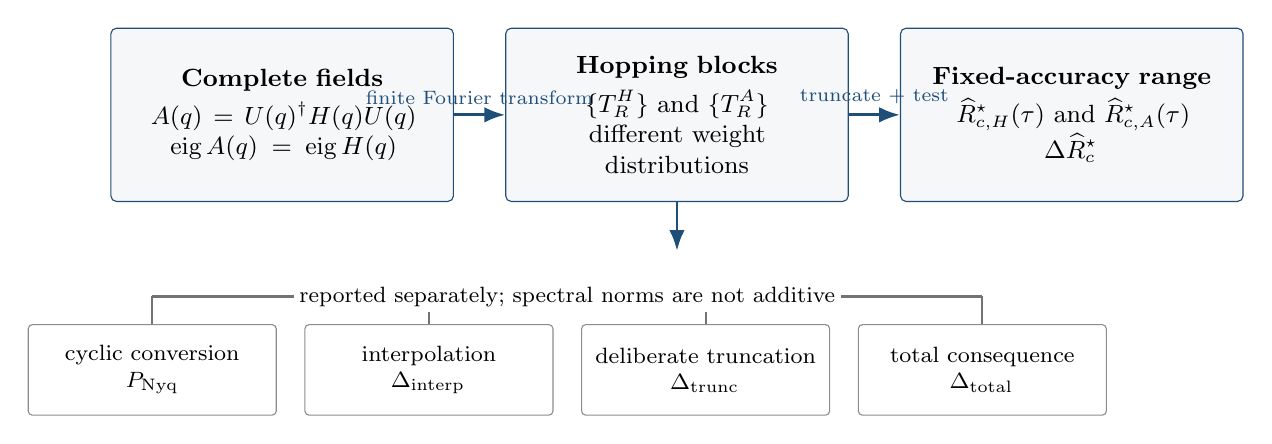
\begin{tikzpicture}[
  >=Latex,
  stage/.style={draw=protocolblue,rounded corners=2pt,fill=protocolgray,
                minimum width=4.35cm,minimum height=2.2cm,align=center,
                font=\small,text width=4.0cm},
  channel/.style={draw=black!45,rounded corners=1.5pt,fill=white,
                  minimum width=3.15cm,minimum height=1.15cm,align=center,
                  font=\footnotesize,text width=2.85cm},
  arrow/.style={->,line width=1pt,protocolblue},
  link/.style={line width=0.8pt,black!55}
]
  \node[stage] (complete) {
    \textbf{Complete fields}\\[1mm]
    $A(q)=U(q)^\dagger H(q)U(q)$\\
    $\operatorname{eig}A(q)=\operatorname{eig}H(q)$
  };
  \node[stage,right=0.65cm of complete] (fourier) {
    \textbf{Hopping blocks}\\[1mm]
    $\{T_R^H\}$ and $\{T_R^A\}$\\
    different weight distributions
  };
  \node[stage,right=0.65cm of fourier] (accuracy) {
    \textbf{Fixed-accuracy range}\\[1mm]
    $\widehat R_{c,H}^\star(\tau)$ and
    $\widehat R_{c,A}^\star(\tau)$\\
    $\Delta\widehat R_c^\star$
  };
  \draw[arrow] (complete) -- (fourier)
    node[midway,above,font=\scriptsize] {finite Fourier transform};
  \draw[arrow] (fourier) -- (accuracy)
    node[midway,above,font=\scriptsize] {truncate + test};

  \node[channel,below=1.55cm of complete,xshift=-1.65cm] (conversion) {
    cyclic conversion\\$P_{\mathrm{Nyq}}$
  };
  \node[channel,right=0.35cm of conversion] (interpolation) {
    interpolation\\$\Delta_{\mathrm{interp}}$
  };
  \node[channel,right=0.35cm of interpolation] (truncation) {
    deliberate truncation\\$\Delta_{\mathrm{trunc}}$
  };
  \node[channel,right=0.35cm of truncation] (total) {
    total consequence\\$\Delta_{\mathrm{total}}$
  };
  \draw[link] (conversion.north) -- ++(0,0.35);
  \draw[link] (interpolation.north) -- ++(0,0.35);
  \draw[link] (truncation.north) -- ++(0,0.35);
  \draw[link] (total.north) -- ++(0,0.35);
  \draw[link] ($(conversion.north)+(0,0.35)$)
    -- ($(total.north)+(0,0.35)$);
  \draw[arrow] (fourier.south) -- ++(0,-0.62);
  \node[font=\footnotesize,fill=white,inner sep=2pt]
    at ($(interpolation.north)!0.5!(truncation.north)+(0,0.35)$)
    {reported separately; spectral norms are not additive};
\end{tikzpicture}
\caption{Logical structure of the benchmark. Momentum-dependent unitary similarity
preserves the complete Bloch spectrum but changes the hopping representation. Explicit
ordinary-lattice truncation then converts that representation difference into a
measurable range requirement at fixed sampled band accuracy. The four approximation
channels are evaluated separately rather than stacked into an additive error budget.}
\label{fig:mechanism}
\end{figure*}

\subsection{Finite-range periodic realization}

\subsubsection{Finite-range parent Hamiltonian}

The controlled parent is a one-dimensional periodic model with lattice period $a_0$ and
four states per cell. Let $k$ denote the physical Bloch wavenumber and
$G=2\pi/a_0$ the primitive reciprocal-lattice magnitude. The calculation uses the
dimensionless reduced coordinate
\begin{equation}
 q=\frac{k}{G}=\frac{k a_0}{2\pi},
 \qquad -\frac12\le q<\frac12.
 \label{eq:reduced-wavenumber}
\end{equation}
Thus $k$ has units of inverse length, whereas $q$ is expressed in reciprocal-lattice
units. The reduced coordinate is used below because lattice translations then enter as
$e^{2\pi iqR}$ with integer cell displacement $R$. The four states are grouped into a
lower two-orbital sector and an upper two-orbital sector. In
this block convention, the nonzero hopping matrices are
\begin{align}
 T_0&=
 \begin{pmatrix}
 D_{\mathrm L}&0\\
 0&D_{\mathrm U}
 \end{pmatrix},\nonumber\\
 T_{+1}&=
 \begin{pmatrix}
 J_{\mathrm L}&V\\
 0&J_{\mathrm U}
 \end{pmatrix},
 &T_{-1}&=T_{+1}^\dagger.
 \label{eq:parent-hopping-blocks}
\end{align}
We measure energy in an arbitrary positive scale $E_{\mathrm{ref}}$. It is a
normalization constant, not a band gap. The $2\times2$ blocks are
\begin{align}
 D_{\mathrm L}&=
 \begin{pmatrix}-1.20&0.06\\0.06&-0.35\end{pmatrix},
 &
 D_{\mathrm U}&=
 \begin{pmatrix}1.00&0.04\\0.04&1.75\end{pmatrix},\nonumber\\
 J_{\mathrm L}&=
 \begin{pmatrix}0.15&0\\0&-0.10\end{pmatrix},
 &
 J_{\mathrm U}&=
 \begin{pmatrix}0.05&0\\0&-0.04\end{pmatrix},\nonumber\\
 V&=
 \begin{pmatrix}0.12&0\\0&0.10\end{pmatrix}.
 \label{eq:parent-numerical-blocks}
\end{align}
Thus $D_{\mathrm L}$ and $D_{\mathrm U}$ describe intracell mixing within the lower and
upper sectors, $J_{\mathrm L}$ and $J_{\mathrm U}$ describe nearest-cell hopping within
each sector, and $V$ couples the lower sector in one cell to the upper sector in the
neighboring cell. Hermitian conjugation supplies the reverse coupling.

With $z=e^{2\pi iq}$, the Bloch Hamiltonian is
\begin{align}
 K(q)&=
 \begin{pmatrix}
 D_{\mathrm L}+zJ_{\mathrm L}+z^{-1}J_{\mathrm L}^\dagger & zV\\
 z^{-1}V^\dagger & D_{\mathrm U}+zJ_{\mathrm U}+z^{-1}J_{\mathrm U}^\dagger
 \end{pmatrix},\nonumber\\
 &=\sum_{R=-1}^{1}e^{2\pi iqR}T_R.
 \label{eq:parent-bloch}
\end{align}
These block values define the parent Hamiltonian rather than one particular momentum
sample. All resolution levels evaluate this same parent; refinement changes only the
set of sampled momenta. The model is synthetic rather than material-specific. Its two
internally mixed orbital sectors are separated in onsite energy but coupled across
neighboring cells, producing a momentum-dependent retained subspace with finite hopping
support.

\subsubsection{Conventional Bloch-band solution}
\label{sec:conventional-bloch}

The analysis begins with the standard Bloch calculation. In operator notation, the
cell-periodic Bloch problem is
\begin{equation}
 \widehat K(k)|\psi_{nk}\rangle=\varepsilon_n(k)|\psi_{nk}\rangle,
 \qquad k=qG.
 \label{eq:bloch-eigenproblem}
\end{equation}
In the declared four-orbital cell basis $\{|\chi_{\alpha k}\rangle\}_{\alpha=1}^4$,
Eq.~\eqref{eq:bloch-eigenproblem} becomes
\begin{equation}
 K_{\alpha\beta}(q)
 =\langle\chi_{\alpha k}|\widehat K(k)|\chi_{\beta k}\rangle,
 \qquad
 K(q)y_n(q)=\varepsilon_n(q)y_n(q).
 \label{eq:bloch-matrix-representation}
\end{equation}
At each momentum $q$, the matrix in Eq.~\eqref{eq:parent-bloch} is assembled and this
Hermitian eigenproblem is solved independently. The four eigenvalues are sorted in
ascending order. A
conventional band plot consists of the functions $\varepsilon_a(q)$ sampled along the
reciprocal mesh.

The present reduction retains the two lowest eigenvectors. The gap between the second
and third eigenvalues protects this rank-two subspace from the discarded states. The
calculation stops if that gap is smaller than the prescribed lower bound; it does not
silently change the retained rank or band identity. At this stage, no relation has been
imposed between the eigenvector phases or internal rank-two bases returned at neighboring
momenta. Those choices do not affect a conventional band plot because they do not change
the eigenvalues.

\subsubsection{Smooth periodic frame}

A matrix comparison requires a basis for the retained subspace. Raw eigenvectors from a
numerical eigensolver have arbitrary phases and unconstrained rotations within the
retained rank-two space. The calculation therefore constructs a \emph{discrete parallel-transport gauge}
around the reciprocal period. In plain terms, the transport visits momentum points in
order:
\[
 q_0\longrightarrow q_1\longrightarrow q_2\longrightarrow\cdots.
\]
At each new point, the raw eigensolver basis is rotated to match the already accepted
basis at the preceding point as closely as possible. This removes arbitrary phase
changes and basis rotations introduced independently by the eigensolver. Operationally,
the procedure is neighbor-to-neighbor SVD/Procrustes alignment. This step fixes the
basis convention within the retained subspace; the subspace itself and its spectrum are
unchanged.

Let $|y_{nq_i}\rangle$ denote the raw cell-periodic Bloch eigenstates returned for the
two retained bands, and let $|f_{nq_i}\rangle$ denote the transported cell-periodic
Bloch frame accepted at that point. Collect these kets as the columns of
$Y_i\in\C^{4\times2}$ and $F_i\in\C^{4\times2}$, respectively. Here $q=k/G$ is the
reduced crystal momentum, so a physical one-dimensional wave vector is $k=qG$.
Both frames have orthonormal columns. The $2\times2$ matrix
\begin{equation}
 M_i=F_i^\dagger Y_{i+1}
 \label{eq:neighbor-overlap}
\end{equation}
is the \emph{neighbor-overlap matrix}; its entries are
$[M_i]_{mn}=\langle f_{mq_i}|y_{nq_{i+1}}\rangle$. The resulting finite Procrustes
problem is the usual Bloch-frame gauge alignment between neighboring momenta.

Write its singular-value decomposition as
\begin{align}
 M_i&=L_i\Sigma_iR_i^\dagger,
 &\Sigma_i&=\operatorname{diag}(\sigma_{i,1},\sigma_{i,2}),\nonumber\\
 &&1&\ge\sigma_{i,1}\ge\sigma_{i,2}\ge0.
 \label{eq:overlap-svd}
\end{align}
The singular values measure the overlap of the two retained subspaces along their two
principal directions. A value near one indicates a well-matched direction; a value near
zero indicates that one direction at $q_{i+1}$ has almost no overlap with the retained
space at $q_i$.

Starting from $F_0=Y_0$, the next accepted frame is
\begin{equation}
 F_{i+1}=Y_{i+1}Q_i,
 \qquad
 Q_i=R_iL_i^\dagger.
 \label{eq:parallel-transport}
\end{equation}
The unitary matrix $Q_i$ is the rotation that makes the new frame as close as possible
to $F_i$ in the Frobenius norm; explicitly,
\begin{equation}
 Q_i=\underset{Q^\dagger Q=I}{\operatorname{argmin}}
 \;\norm{Y_{i+1}Q-F_i}_F.
 \label{eq:neighbor-procrustes-objective}
\end{equation}
It changes only the coordinate basis inside the retained subspace; it neither changes the
subspace nor refits the Hamiltonian. This is the singular-value form of unitary polar or
Procrustes alignment. The real orthogonal least-squares formulation is derived by
Sch\"onemann~\cite{schonemann1966}. For the complex unitary form used here, Higham's
Eqs.~(2.1)--(2.3) construct the unitary polar factor from the singular-value
decomposition, and Theorem~2.2, in particular inequality~(2.4), gives its
Frobenius-norm optimality~\cite{higham1986}. The aligned neighbor overlap
$F_i^\dagger F_{i+1}$ is Hermitian positive semidefinite.

The protocol introduces a minimum allowed singular value $\sigma_{\mathrm{rank}}$. The
draft value is $0.8$; the final value must be recorded in canonical input. Each step must
satisfy
\begin{equation}
 \sigma_{i,2}>\sigma_{\mathrm{rank}}.
 \label{eq:overlap-rank-test}
\end{equation}
If this test fails, the basis at the next point is not sufficiently determined by its
overlap with the preceding basis, and the calculation stops.

To state the uniqueness issue explicitly, the polar decomposition of the overlap is
$M_i=P_iH_i$, where $P_i=L_iR_i^\dagger$ is unitary and
$H_i=R_i\Sigma_iR_i^\dagger$ is Hermitian positive semidefinite. The applied rotation is
$Q_i=P_i^\dagger$. When both singular values are positive, $P_i$ and therefore $Q_i$ are
unique. If a singular value is zero, rotations acting within the corresponding null
directions cannot be inferred from $M_i$; several equally optimal choices exist. The
calculation rejects that case rather than selecting one of those choices. This is the
full-rank uniqueness condition in Higham's Theorem~1.1~\cite{higham1986}.

Discrete parallel transport generally leaves a residual mismatch across the periodic boundary.
To define that mismatch without an orientation ambiguity, append the duplicate endpoint
$Y_N=Y_0$ and apply the same full-rank Procrustes step from $F_{N-1}$ to obtain $F_N$.
Reduce $S=F_0^\dagger F_N$ to its unitary polar factor. If
$S=Z\,\operatorname{diag}(e^{i\gamma_1},e^{i\gamma_2})Z^\dagger$, with principal phases
$\gamma_j\in(-\pi,\pi]$, distribute the residual mismatch over the periodic extension by
\begin{align}
 W_i&=Z\,\operatorname{diag}
 \left(e^{-i(i/N)\gamma_1},e^{-i(i/N)\gamma_2}\right)Z^\dagger,\nonumber\\
 F_i&\leftarrow F_iW_i,
 \qquad i=0,\ldots,N.
 \label{eq:closure-correction}
\end{align}
The corrected duplicate endpoint must agree with the corrected start, and all retained
sample frames $i=0,\ldots,N-1$ must satisfy orthonormality and retained-projector
reconstruction checks. Proximity to the phase branch cut is recorded as a numerical
diagnostic.

The frame remains qualified by the eigensolver and linear-algebra backend that produced
it. The protocol does not assert a canonical frame shared by all backends. Projectors,
reconstructed operators, and independently verified observables carry the invariant
meaning.

\subsubsection{Reference and comparison matrices}

The retained reference matrix is
\begin{equation}
 H(q_i)=F_i^\dagger K(q_i)F_i.
 \label{eq:reference-matrix}
\end{equation}
The dispersive realization uses the same smooth one-parameter family as the flat
benchmark. Define
\begin{align}
 \theta_a(q)&=a\sin(2\pi q),\\
 U_a(q)&=
 \begin{pmatrix}
 \cos\theta_a(q)&-\sin\theta_a(q)\\
 \sin\theta_a(q)& \cos\theta_a(q)
 \end{pmatrix},\\
 A_a(q)&=U_a(q)^\dagger H(q)U_a(q),
 \qquad 0\le a\le\frac\pi4.
 \label{eq:attacked-matrix}
\end{align}
By construction, $A_a(q)$ and $H(q)$ have identical ordered eigenvalues. They are treated
as matrix fields in the common retained coordinates defined by $F(q)$. The admissible
identification permits one subsequent global real rotation and excludes reuse of the
generating momentum-dependent $U_a(q)$. The resulting loss is therefore a
restricted-alignment representation error, not a claim that the two fields cease to be
unitarily equivalent as abstract operators. Their Fourier hopping blocks generally
differ in the declared coordinates.

The earlier fixed finite-angle field belongs only to the isolated historical regression
fixture. Its coefficients are not controls of either active smooth realization.

\subsection{Candidate family and allowed alignment}

\subsubsection{Positive trace--traceless affine deformation}

Write the retained reference matrix as
\begin{align}
 H(q)&=\bar E(q)I_2+D(q),
 &\bar E(q)&=\frac12\operatorname{tr}H(q),\nonumber\\
 &&\operatorname{tr}D(q)&=0.
 \label{eq:trace-decomposition}
\end{align}
The candidate family is
\begin{equation}
 C_{s,\lambda}(q)
 =\bar E(q)I_2+sE_{\mathrm{ref}}I_2+\lambda D(q),
 \qquad \lambda>0.
 \label{eq:candidate}
\end{equation}
This is the \emph{positive trace--traceless affine deformation family}. Equivalently,
it is an energy-centroid shift followed by a rescaling of the level splitting. The
parameter $s$ translates both retained energy levels by $sE_{\mathrm{ref}}$, while $\lambda$ rescales
their displacement from the mean. Positivity of $\lambda$ preserves the ordering of the
two levels.

If $h_1(q)\le h_2(q)$ are the eigenvalues of $H(q)$, the candidate eigenvalues are known
without a further eigensolve:
\begin{equation}
 c_a(q;s,\lambda)
 =\bar E(q)+sE_{\mathrm{ref}}+\lambda[h_a(q)-\bar E(q)].
 \label{eq:candidate-eigenvalues}
\end{equation}
The parameter vector $p=(s,\lambda)^T$ is restricted to a closed rectangle
\begin{equation}
 X=[s_{\min},s_{\max}]
 \times[\lambda_{\min},\lambda_{\max}],
 \qquad \lambda_{\min}>0.
 \label{eq:parameter-box}
\end{equation}
The four bounds affect the scientific outcome and must be fixed before confirmatory
execution.

\subsubsection{Continuous global alignment family}

The operator comparison allows one global real rotation
\begin{align}
 R(\phi)&=
 \begin{pmatrix}
 \cos\phi&-\sin\phi\\
 \sin\phi& \cos\phi
 \end{pmatrix},\nonumber\\
 C_{s,\lambda,\phi}(q)
 &=R(\phi)^\dagger C_{s,\lambda}(q)R(\phi).
 \label{eq:global-alignment}
\end{align}
The same angle is used at every momentum. Momentum-dependent and unrestricted complex
unitary transformations are outside the claim. Since conjugation by
$R(\phi+\pi)=-R(\phi)$ is unchanged, the continuous fundamental interval is
\begin{equation}
 -\frac\pi2\le\phi<\frac\pi2.
 \label{eq:continuous-angle-domain}
\end{equation}
The optimum over this interval is calculated analytically from the second-harmonic
correlation derived below. No finite angle inventory defines the result. This restricted
cross-representation alignment is not MLWF gauge optimization: it does not minimize a
Wannier spread, and it deliberately excludes the generating momentum-dependent
transformation from the admissible comparison family.

\subsection{Exact quadratic theory}

\subsubsection{Loss definitions}

Let $q_i$ be a construction coordinate and $w_i>0$ its raw objective weight. Define
\[
 \alpha_i=\frac{w_i}{\sum_jw_j}.
\]
The canonical input stores the raw weights. A prospective exclusion rule is the only
valid way to omit a coordinate; a zero weight is not a substitute for exclusion.

For retained rank two, the spectral loss and restricted-alignment matrix loss
(the operator channel) are
\begin{align}
 L_{\mathrm{spec}}^2(s,\lambda)
 &=\sum_i\frac{\alpha_i}{2}
   \sum_{n=1}^{2}
   \left|
   \frac{c_n(q_i;s,\lambda)-h_n(q_i)}{E_{\mathrm{ref}}}
   \right|^2,
 \label{eq:spectral-loss}\\
 L_{\mathrm{op},\phi}^2(s,\lambda)
 &=\sum_i\frac{\alpha_i}{2}
   \left\lVert
   \frac{C_{s,\lambda,\phi}(q_i)-A_a(q_i)}{E_{\mathrm{ref}}}
   \right\rVert_F^2.
 \label{eq:operator-loss}
\end{align}
To connect the matrix loss to the Bloch states, define the retained-space residual
operator
$\widehat{\Delta H}_{s,\lambda,\phi,a}(k_i)
 =\widehat C_{s,\lambda,\phi}(k_i)-\widehat A_a(k_i)$. In the transported Bloch frame,
\begin{equation}
 [C_{s,\lambda,\phi}(q_i)-A_a(q_i)]_{mn}
 =\langle f_{mq_i}|\widehat{\Delta H}_{s,\lambda,\phi,a}(k_i)
  |f_{nq_i}\rangle.
 \label{eq:operator-residual-bloch-matrix-element}
\end{equation}
Hence the operator channel is the Brillouin-zone root-mean-square of all retained
Bloch-Hamiltonian matrix-element errors rather than merely an eigenvalue error. Here and
throughout,
\begin{equation}
 \norm{M}_F^2=\operatorname{tr}(M^\dagger M)=\sum_{m,n}|M_{mn}|^2
 \label{eq:frobenius-definition}
\end{equation}
is the squared Frobenius norm: the sum of the squared magnitudes of every matrix entry.
The factor $1/2$ gives a per-retained-state normalization, and division by $E_{\mathrm{ref}}^2$
makes both losses dimensionless.

Define the positive splitting scale
\begin{equation}
 \kappa=
 \sum_i\frac{\alpha_i}{2E_{\mathrm{ref}}^2}\norm{D(q_i)}_F^2.
 \label{eq:kappa}
\end{equation}
The nontrivial case has $\kappa>0$, meaning that the retained Hamiltonian is not a scalar
multiple of the identity at every construction coordinate.

For one declared amplitude $a$, suppress the amplitude index on the comparison target.
For an allowed global angle $\phi$, write
\begin{align}
 D_{i,\phi}&=R(\phi)^\dagger D(q_i)R(\phi),\\
 B_i&=U_a(q_i)^\dagger D(q_i)U_a(q_i),\\
 b_\phi&=
 \sum_i\frac{\alpha_i}{2E_{\mathrm{ref}}^2}
 \operatorname{Re}\operatorname{tr}(D_{i,\phi}^\dagger B_i),\\
 \mu_\phi&=\frac{b_\phi}{\kappa}.
 \label{eq:operator-correlation}
\end{align}
The scalar $\mu_\phi$ is the normalized correlation between the globally aligned
traceless candidate and the momentum-dependent comparison target.

For a traceless Hermitian $2\times2$ matrix, write
\[
 D_i=x_i\sigma_x+y_i\sigma_y+z_i\sigma_z,
 \qquad
 B_i=X_i\sigma_x+Y_i\sigma_y+Z_i\sigma_z.
\]
Conjugation by a real rotation leaves the $\sigma_y$ component fixed and rotates the
$(\sigma_x,\sigma_z)$ components through angle $2\phi$. Consequently,
\begin{equation}
 b_\phi=b_0+c\cos(2\phi)+d\sin(2\phi),
 \label{eq:correlation-harmonic}
\end{equation}
where
\begin{align}
 b_0&=\sum_i\frac{\alpha_i}{E_{\mathrm{ref}}^2}y_iY_i,\\
 c&=\sum_i\frac{\alpha_i}{E_{\mathrm{ref}}^2}(x_iX_i+z_iZ_i),\\
 d&=\sum_i\frac{\alpha_i}{E_{\mathrm{ref}}^2}(x_iZ_i-z_iX_i).
 \label{eq:harmonic-coefficients}
\end{align}
The exact continuous maximum is
\begin{equation}
 b_{\max}=b_0+\sqrt{c^2+d^2},
 \qquad
 \mu_{\max}=\frac{b_{\max}}{\kappa}.
 \label{eq:continuous-correlation-maximum}
\end{equation}
When $c^2+d^2$ exceeds the declared degeneracy cutoff, a canonical maximizing angle is
\begin{equation}
 \phi_*=\frac12\operatorname{atan2}(d,c)
 \quad\text{reduced to}\quad[-\pi/2,\pi/2).
 \label{eq:continuous-maximizing-angle}
\end{equation}
If the harmonic amplitude is numerically zero, every angle is equally optimal; the
maximum value remains defined but no unique angle is reported.

\subsubsection{Common-curvature theorem}

\begin{theorem}[Exact loss geometry]
\label{thm:exact-loss-geometry}
Under Eqs.~\eqref{eq:trace-decomposition}--\eqref{eq:operator-correlation}, the losses are
\begin{align}
 L_{\mathrm{spec}}^2(s,\lambda)
 &=s^2+\kappa(\lambda-1)^2,
 \label{eq:exact-spectral-loss}\\
 L_{\mathrm{op},\phi}^2(s,\lambda)
 &=s^2+\kappa(\lambda-\mu_\phi)^2
   +\kappa(1-\mu_\phi^2),
 \label{eq:exact-operator-loss}
\end{align}
and $|\mu_\phi|\le1$. Consequently, the spectral loss and every operator loss have the
same parameter-space curvature
\begin{equation}
 Q=\begin{pmatrix}1&0\\0&\kappa\end{pmatrix}.
 \label{eq:common-curvature}
\end{equation}
The operator component at angle $\phi$ is centered at $(0,\mu_\phi)$ and has irreducible
minimum $m_\phi=\kappa(1-\mu_\phi^2)$. Because the candidate requires $\lambda>0$,
minimizing over the continuous global alignment is equivalent to maximizing $b_\phi$.
The continuously aligned loss is therefore the single quadratic
\begin{equation}
 L_{\mathrm{op},*}^2(s,\lambda)
 =s^2+\kappa(\lambda-\mu_{\max})^2
  +\kappa(1-\mu_{\max}^2).
 \label{eq:continuously-optimized-operator-loss}
\end{equation}
\end{theorem}

\begin{proof}
A complete derivation is given in Supplementary Sec.~S1.1.
\end{proof}

The theorem identifies the theoretical content of the experiment. Momentum sampling is
needed only to evaluate $\kappa$ and the three harmonic coefficients accurately; it does
not create a collection of independent parent models. The incompatibility mechanism is
$\kappa(1-\mu_{\max}^2)$: it measures the part of the momentum-dependent traceless target
that cannot be represented by one continuously optimized global rotation and one
positive uniform splitting scale.

\subsection{Exact admissible-set geometry}

Let $\tau_s$ and $\tau_o$ be the spectral and operator error limits. Their values must be
fixed from a stated scientific error budget or identified as synthetic benchmark
controls. Define
\begin{align}
 \mathcal A_s
 &=\{p\in X:L_{\mathrm{spec}}(p)\le\tau_s\},\\
 \mathcal A_o
 &=\{p\in X:L_{\mathrm{op},*}(p)\le\tau_o\}.
 \label{eq:admissible-sets}
\end{align}
The operator ellipse radius in the scaled coordinates is
\begin{equation}
 r_*=
 \sqrt{\tau_o^2-\kappa(1-\mu_{\max}^2)}.
 \label{eq:operator-radius}
\end{equation}
The operator admissible set is empty when the radicand is negative.

Each point $p=(s,\lambda)^T$ in these sets denotes one concrete Bloch-Hamiltonian model:
$sE_{\mathrm{ref}}$ is a uniform centroid-energy shift and $\lambda$ is a positive rescaling of the
retained band splitting. Thus $\mathcal A_s$ contains candidates whose band energies
meet the spectral error budget, while $\mathcal A_o$ contains candidates whose retained
Bloch-Hamiltonian matrix elements in the declared frame meet the operator error budget
after one global rotation. A \emph{joint witness} is the same physical candidate
$(s,\lambda)$ belonging to both sets. A separation certificate proves only that no member
of this declared two-parameter candidate family, under the declared global alignment and
error limits, satisfies both requirements. It is not a claim that the complete
Hamiltonians are physically inequivalent, that no larger model class can work, or that a
material phase or topology has been certified. The ellipses live in model-parameter
space, not in the Brillouin zone.

\begin{corollary}[Compatibility and exact full-ellipse distance]
\label{cor:compatibility-distance}
Assume $r_*$ is real and that the spectral and continuously optimized operator ellipses
are contained in the parameter rectangle $X$. They intersect if and only if
\begin{equation}
 \sqrt{\kappa}\,|1-\mu_{\max}|
 \le \tau_s+r_*.
 \label{eq:exact-intersection}
\end{equation}
Their Euclidean distance in $(s,\lambda)$ coordinates is
\begin{equation}
 \delta_*=
 \max\left\{0,
 |1-\mu_{\max}|-\frac{\tau_s+r_*}{\sqrt{\kappa}}
 \right\}.
 \label{eq:exact-distance}
\end{equation}
\end{corollary}

\begin{proof}
A complete derivation is given in Supplementary Sec.~S1.2.
\end{proof}

Thus the theoretical decision is explicit. A common witness exists exactly when
Eq.~\eqref{eq:exact-intersection} holds. Strict separation holds for the full ellipses
when that inequality fails; a resolution-qualified claim additionally requires
\begin{equation}
 \delta_*>\rho_{\mathrm{sep}}
 \label{eq:resolution-qualified-separation}
\end{equation}
with a numerical uncertainty margin.

The containment premise is explicit. The formulas above describe full ellipses, not
ellipses clipped by $X$. The calculation verifies every coordinate extremum before using
the corollary as the declared certificate. Failed containment produces an
\emph{invalid premise} or \emph{unresolved} record; it never triggers an implicit
box-clipped substitute.

For numerical verification, a general quadratic is still retained in the form
\begin{align}
 r(p)&=r_0+\mathsf Jp,
 &L^2(p)&=p^TQp+2g^Tp+c,\nonumber\\
 Q&=\operatorname{Re}(\mathsf J^\dagger W\mathsf J),
 &g&=\operatorname{Re}(\mathsf J^\dagger Wr_0),\nonumber\\
 c&=\operatorname{Re}(r_0^\dagger Wr_0).
 \label{eq:quadratic}
\end{align}
Here $r_0$ is the stacked complex residual at $p=0$, $\mathsf J$ is its affine
parameter-response matrix, and $W$ contains the declared momentum, retained-state, and
energy-scale weights. For the spectral channel the stacked entries are Bloch-energy
residuals; for the operator channel they are the Bloch-frame matrix elements in
Eq.~\eqref{eq:operator-residual-bloch-matrix-element}. Thus the generic quadratic is an
algebraic representation of the stated Bloch residuals, not a separate fitted model.
The independently reconstructed coefficients must agree with the analytic structure in
Theorem~\ref{thm:exact-loss-geometry}: vanishing cross curvature, unit shift curvature,
common splitting curvature $\kappa$, spectral center $(0,1)$, continuous operator center
$(0,\mu_{\max})$, and agreement of the retained maximizing angle with
Eq.~\eqref{eq:continuous-maximizing-angle}. These identities provide stronger
verification than merely fitting a quadratic to sampled loss values.

\subsection{Operator information omitted by the Bloch spectrum}

The conventional calculation in Section~\ref{sec:conventional-bloch} retains the
ordered eigenvalues. Applied to the controlled pair $H(q)$ and $A_a(q)$, it finds exact
agreement because
\[
 A_a(q)=U_a(q)^\dagger H(q)U_a(q)
\]
is a unitary conjugation at every momentum. In the candidate family, the same statement
appears as
\begin{equation}
 L_{\mathrm{spec}}(0,1)=0.
 \label{eq:conventional-band-result}
\end{equation}
Thus a band-only calculation accepts the undeformed candidate independently of how
strongly $U(q)$ varies with momentum.

The restricted-alignment matrix question contains information discarded by that
comparison. After exact continuous maximization of the global angle,
Theorem~\ref{thm:exact-loss-geometry} gives the unconstrained best operator residual
\begin{equation}
 \inf_{s\in\mathbb R,\,\lambda\ge0}L_{\mathrm{op},*}^2(s,\lambda)
 =\kappa\left[1-\max(0,\mu_{\max})^2\right].
 \label{eq:operator-blind-spot}
\end{equation}
A strictly positive lower splitting bound only increases this infimum.
When the momentum-dependent comparison field is exactly representable by one global
rotation, $\mu_{\max}=1$ and the residual vanishes at $(s,\lambda)=(0,1)$. Otherwise,
$1-\mu_{\max}^2$ quantifies the part that a conventional band comparison cannot see and
a single global alignment cannot reproduce.

The same distinction appears in real space. If
\[
 H(q)=\sum_R e^{2\pi iqR}T_R,
 \qquad
 U(q)=\sum_m e^{2\pi iqm}U_m,
\]
then the hopping blocks of $A(q)=U(q)^\dagger H(q)U(q)$ are
\begin{equation}
 \widetilde T_Q=
 \sum_{m,n}U_m^\dagger T_{Q+m-n}U_n.
 \label{eq:gauge-hopping-convolution}
\end{equation}
A momentum-independent basis change has only one nonzero Fourier coefficient and
conjugates each hopping block without changing its range. A momentum-dependent change
mixes displacement indices through Eq.~\eqref{eq:gauge-hopping-convolution}, redistributing
weight to longer-range blocks while leaving every band energy unchanged.

The comparison is therefore not between two ways of computing the same band structure.
The conventional calculation answers whether the energies agree. The present theory
asks the stronger question of whether the same restricted candidate also reproduces the
Hamiltonian in a declared frame and the associated hopping representation. The scalar
$\mu_{\max}$ is the exact bridge between those questions for the rank-two family.

\subsubsection{An exact band-only false positive}

The theory permits an explicit construction in which the conventional band criterion
passes exactly while joint spectral and operator adequacy fails by a positive margin.
This is an analytic counterexample, not a calculated outcome for the four-state parent.

\begin{proposition}[Exact spectral pass with certified operator incompatibility]
\label{prop:constructed-fail}
Consider two equally weighted momentum observations with
\[
 H_1=H_2=\bar E I_2+E_{\mathrm{ref}}\sigma_z,
 \qquad
 \sigma_z=\begin{pmatrix}1&0\\0&-1\end{pmatrix},
\]
and comparison rotations
\[
 U_1=R(0),
 \qquad
 U_2=R(\pi/4).
\]
Allow every global real rotation $R(\phi)$ and choose
\begin{align*}
 X&=[-0.20,0.20]\times[0.50,1.10],\\
 \tau_s&=0.05,
 &\tau_o&=0.72.
\end{align*}
Then the conventional spectral loss vanishes at $(s,\lambda)=(0,1)$, but no point in
$X$ satisfies both error limits. The Euclidean separation of the closest full
admissible ellipses is
\begin{equation}
 \delta_*
 =1-\frac{1}{\sqrt2}-0.05
  -\sqrt{0.72^2-\frac12}
 \approx0.1072466192.
 \label{eq:constructed-fail-distance}
\end{equation}
Consequently, any declared separation resolution
$\rho_{\mathrm{sep}}<\delta_*$ is certified.
\end{proposition}

\begin{proof}
A complete derivation is given in Supplementary Sec.~S1.3.
\end{proof}

This construction states precisely what ``the bands pass but the reduced Hamiltonian
fails'' means. The failure is not an optimizer failure: it follows from the exact loss
geometry and a positive certified distance between admissible sets.

\subsubsection{A smooth continuum of band-equivalent Hamiltonians}

For comparison across the complete reciprocal period, use the smooth periodic family
already defined in Eq.~\eqref{eq:attacked-matrix}:
\begin{equation}
 \begin{split}
 \mathcal U_{\mathrm{smooth}}=\bigl\{U_a(q)&=R\!\left(a\sin 2\pi q\right):\\
 &0\le a\le\pi/4\bigr\}.
 \end{split}
 \label{eq:attack-continuum}
\end{equation}
The parameter $a$ is the maximum basis-rotation amplitude. At $a=0$, the comparison and
reference matrices coincide. Increasing $a$ introduces progressively stronger
momentum-to-momentum basis variation while preserving every Bloch eigenvalue exactly.
Unlike a piecewise rotation, Eq.~\eqref{eq:attack-continuum} is smooth and periodic, so
its induced hopping tail reflects a controlled Fourier hierarchy rather than a jump
discontinuity.

For the flat traceless rank-two parent in Eq.~\eqref{eq:flat-traceless-parent}, the
Jacobi--Anger expansion gives the reciprocal-period average
\begin{equation}
 \mu_{\max}(a)=J_0(2a),
 \label{eq:continuum-correlation}
\end{equation}
where $J_0$ is the Bessel function of the first kind~\cite[Sec.~10.12]{dlmf1012}.

\begin{corollary}[Smooth monotone threshold continuum]
\label{cor:threshold-continuum}
For the family in Eq.~\eqref{eq:attack-continuum}, before finite parameter bounds are
applied, the infimum operator threshold is
\begin{equation}
 \tau_{o,\min}(a)
 =\sqrt{\kappa\left[1-J_0(2a)^2\right]}.
 \label{eq:minimum-operator-threshold}
\end{equation}
For a fixed spectral threshold $\tau_s$, the smallest operator threshold permitting a
joint witness is
\begin{align}
 \tau_{o,\mathrm{joint}}(a;\tau_s)^2
 &=\kappa\left[1-J_0(2a)^2\right]\nonumber\\
 &\quad+\max\!\left\{0,
   \sqrt{\kappa}\left[1-J_0(2a)\right]-\tau_s
  \right\}^{2}.
 \label{eq:joint-threshold-continuum}
\end{align}
For exact spectral acceptance this reduces to
\begin{equation}
 \tau_{o,\mathrm{joint}}(a;0)
 =\sqrt{2\kappa\left[1-J_0(2a)\right]}.
 \label{eq:exact-spectrum-threshold-continuum}
\end{equation}
All three quantities are nondecreasing on $0\le a\le\pi/4$.
\end{corollary}

\begin{proof}
A complete derivation is given in Supplementary Sec.~S1.4.
\end{proof}

\begin{figure*}[t]
\centering
\begin{tikzpicture}
\begin{axis}[
  width=0.78\textwidth,
  height=0.43\textwidth,
  xmin=0,xmax=0.7853981633974483,
  ymin=0,ymax=1.05,
  xlabel={maximum basis-rotation amplitude $a$},
  ylabel={threshold divided by $\sqrt{\kappa}$},
  xtick={0,0.2617993877991494,0.5235987755982988,0.7853981633974483},
  xticklabels={$0$,$\pi/12$,$\pi/6$,$\pi/4$},
  legend style={at={(0.03,0.97)},anchor=north west,draw=none,fill=white},
  axis lines=left,
  grid=major,
  grid style={black!10}
]
\addplot[protocolblue,very thick]
 table[x=a,y=operator_threshold_over_sqrt_kappa,col sep=comma]
 {../../../../../experiments/model-adequacy/periodic1d/band-equivalence-versus-hopping-locality/smooth-threshold-continuum.csv};
\addlegendentry{$\tau_{o,\min}/\sqrt\kappa$}
\addplot[red!70!black,very thick,dashed]
 table[x=a,y=joint_threshold_over_sqrt_kappa,col sep=comma]
 {../../../../../experiments/model-adequacy/periodic1d/band-equivalence-versus-hopping-locality/smooth-threshold-continuum.csv};
\addlegendentry{$\tau_{o,\mathrm{joint}}(a;0)/\sqrt\kappa$}
\end{axis}
\end{tikzpicture}
\caption{Analytic acceptance thresholds for the smooth continuum in
Eq.~\eqref{eq:attack-continuum}. Every amplitude has exactly the same Bloch bands. The
solid curve is the smallest threshold admitting an operator fit before finite parameter
bounds are applied. The dashed curve additionally requires exact spectral agreement.
The plotted points are evaluations of the displayed Bessel formulas, not empirical
data.}
\label{fig:threshold-continuum}
\end{figure*}

This family supports a direct side-by-side calculation across $a$: the conventional
branch reports zero band change, while the representation-aware branch reports the
operator threshold and the induced Fourier hopping tail.

\subsection{Exact relation to representation-induced hopping range}

The threshold has a direct real-space meaning. Consider the spectrally flat traceless
parent
\begin{align}
 H(q)&=\bar E I_2+D,
 &D&=D^T\in\mathbb R^{2\times2},\nonumber\\
 &&\operatorname{tr}D&=0,
 \qquad D\ne0.
 \label{eq:flat-traceless-parent}
\end{align}
where $\bar E$ and $D$ are independent of momentum. Its only hopping block is onsite.
After a momentum-dependent real rotation, the traceless comparison field is
\begin{equation}
 B(q)=U(q)^\dagger D U(q).
 \label{eq:rotated-traceless-field}
\end{equation}
Define its Fourier blocks by
\begin{equation}
 B_R=\int_{-1/2}^{1/2}e^{-2\pi iqR}B(q)\,dq,
 \qquad
 B(q)=\sum_{R\in\mathbb Z}e^{2\pi iqR}B_R.
 \label{eq:continuous-traceless-fourier}
\end{equation}
The nonzero-$R$ blocks are hopping terms created entirely by the momentum dependence of
the basis transformation.

\begin{theorem}[Operator residual equals induced nonlocal hopping weight]
\label{thm:residual-locality-identity}
Let $B(q)$ be given by Eq.~\eqref{eq:rotated-traceless-field}, with $U(q)$ restricted to
the same real two-dimensional rotation family as the allowed global alignment. Set
\begin{equation}
 \kappa=\frac{\norm{D}_F^2}{2E_{\mathrm{ref}}^2},
 \qquad
 \mu_{\max}=\frac{\norm{B_0}_F}{\norm{D}_F}.
 \label{eq:locality-kappa-mu}
\end{equation}
Then
\begin{align}
 \inf_{s\in\mathbb R,\,\lambda\ge0,\,\phi}
 L_{\mathrm{op},\phi}^2(s,\lambda)
 &=\kappa(1-\mu_{\max}^2)
 \label{eq:residual-locality-left}\\
 &=\frac{1}{2E_{\mathrm{ref}}^2}
   \sum_{R\ne0}\norm{B_R}_F^2.
 \label{eq:residual-locality-right}
\end{align}
Thus the squared irreducible operator residual is exactly the normalized Fourier weight
outside the onsite block. For a finite uniform mesh, the same identity holds with the
integral and Fourier series replaced by the corresponding discrete transform.
\end{theorem}

\begin{proof}
A complete derivation is given in Supplementary Sec.~S1.5.
\end{proof}

For the smooth continuum in Eq.~\eqref{eq:attack-continuum},
$\mu_{\max}(a)=J_0(2a)$. The theorem therefore gives
\begin{equation}
 \frac{1}{2E_{\mathrm{ref}}^2}\sum_{R\ne0}\norm{B_R(a)}_F^2
 =\kappa\left[1-J_0(2a)^2\right]
 =\tau_{o,\min}(a)^2.
 \label{eq:continuum-tail-identity}
\end{equation}
The solid curve in Fig.~\ref{fig:threshold-continuum} is consequently the square root of
the induced non-onsite hopping weight. If exact spectral agreement additionally fixes
$\lambda=1$, the joint threshold contains a second contribution from the mismatch of
the onsite block:
\begin{align}
 \tau_{o,\mathrm{joint}}(a;0)^2
 &=\underbrace{\kappa\left[1-J_0(2a)^2\right]}_{\text{non-onsite hopping weight}}\nonumber\\
 &\quad+\underbrace{\kappa\left[1-J_0(2a)\right]^2}_{\text{onsite-block mismatch}}.
 \label{eq:joint-threshold-locality-decomposition}
\end{align}

This identity is the substantive distinction from a band-only diagnostic. The band
energies remain unchanged, but the momentum-dependent representation necessarily moves
a calculable amount of operator weight outside the cell-local block. A global rotation
changes the orbital basis within each cell but cannot remove those nonzero-range
Fourier blocks.

\section{Methods}

\subsection{Numerical experiment design}

The computational study evaluates the same continuum through two branches. Both branches
start from one solution of the parent Bloch eigenproblem. The parent is not refitted or
rediagonalized as a different physical model at each amplitude.

\subsubsection{Conventional Bloch branch}

For every amplitude $a$ and momentum $q_i$, construct $A_a(q_i)$ from
Eq.~\eqref{eq:attack-continuum} and independently diagonalize it. Record the ordered-band
discrepancy
\begin{equation}
 \Delta_{\mathrm{band}}(a)
 =\max_{i,n}
 \frac{|\varepsilon_n[A_a(q_i)]-\varepsilon_n[H(q_i)]|}{E_{\mathrm{ref}}}.
 \label{eq:band-continuum-discrepancy}
\end{equation}
The analytic value is zero for every $a$; the calculated value measures only numerical
eigensolver and ordering error. The branch also records the two overlaid band curves at
selected amplitudes. No operator matrix element or hopping block enters its acceptance
criterion.

\subsubsection{Representation-aware branch}

Using the same matrices $A_a(q_i)$, calculate
\begin{enumerate}
  \item the best global alignment correlation $\mu_{\max}(a)$;
  \item the irreducible operator loss
        $L_{\mathrm{op,min}}(a)$;
  \item the operator threshold required for a joint witness at each declared spectral
        threshold;
  \item the Fourier hopping blocks $\widetilde T_R(a)$; and
  \item the range-resolved tail
        \begin{equation}
        P_{>R_c}(a)=\frac{1}{2E_{\mathrm{ref}}^2}
        \sum_{|R|>R_c}\norm{\widetilde T_R(a)}_F^2.
        \label{eq:continuum-hopping-tail}
        \end{equation}
\end{enumerate}
For the flat analytic parent, $R_c=0$ and
\begin{equation}
 L_{\mathrm{op,min}}(a)^2=P_{>0}(a)
 =\kappa\left[1-J_0(2a)^2\right].
 \label{eq:continuum-three-way-identity}
\end{equation}
The calculation retains the discrepancy in this three-way identity as a verification channel.
For the finite-range four-state realization, the parent itself has nonzero-range blocks;
the analysis therefore reports the complete range-resolved distribution and its change
with $a$, without assuming that Eq.~\eqref{eq:continuum-three-way-identity} continues to
hold unchanged.

\subsubsection{Continuum evaluation and comparison figures}

The amplitude interval is $0\le a\le\pi/4$. For the flat parent, the continuous
correlation and thresholds are evaluated directly at any requested amplitude from
\begin{equation}
 \mu_{\max}(a)=J_0(2a),\qquad
 \tau_{o,\min}(a)=\sqrt{\kappa[1-J_0(2a)^2]},
 \label{eq:direct-amplitude-evaluation}
\end{equation}
together with Eq.~\eqref{eq:exact-spectrum-threshold-continuum}. No piecewise-linear
amplitude interpolant enters an analytic claim. A diagnostic uniform-grid test through
$N_a=64$ was rejected rather than promoted to a convergence rule: its midpoint errors
exceeded the draft tolerance, whereas direct evaluation has no between-node
interpolation error.

The non-flat parent has no corresponding $J_0(2a)$ comparator. Its numerical statements
are therefore pointwise at the 65 directly evaluated amplitudes used for momentum
refinement or the 33 amplitudes used for the parent and truncation studies. Connecting
lines are guides to the eye, not continuous-amplitude reconstructions. A deterministic
adaptive action remains available if a future claim requires between-node control: it
caches direct samples, refines only failing midpoint intervals, requires disjoint
quarter-point validation, and fails closed at explicit caps. No such continuous non-flat
claim is made here.

Supplementary Fig.~S4 places the direct analytic correlation and thresholds beside
conventional Bloch bands, cumulative tails, and range-resolved hopping weight. The bands
remain unchanged while the representation-aware channels resolve the increasing
operator mismatch and induced hopping range.

\subsection{Fourier reconstruction and locality}

For the selected construction mesh, the matrix-valued forward transform is
\begin{equation}
 T_R^{(N_*)}=\frac{1}{N_*}\sum_{i=0}^{N_*-1}
 e^{-2\pi iq_iR}H(q_i),
 \label{eq:forward-fourier}
\end{equation}
and the finite trigonometric interpolant is
\begin{equation}
 H_{N_*}(q)=\sum_R e^{+2\pi iqR}T_R^{(N_*)}.
 \label{eq:inverse-fourier}
\end{equation}
The identity $H_{N_*}(q_i)=H(q_i)$ holds at the construction nodes. Away from those
nodes, $H_{N_*}$ is a finite interpolant and is not substituted for the continuous field
without an explicit interpolation or convergence check~\cite{trefethen2000,higham2002}. The displacement inventory uses
centered integer representatives of the finite cyclic mesh. For an even mesh, the
Nyquist representative is $-N_*/2$; Hermitian symmetry there is interpreted cyclically,
so its block must be Hermitian. The calculation and verifier must share this convention.

For maximum retained range $R_c$, the finite-mesh omitted-block locality norm is
\begin{equation}
 \eta_{N_*}(R_c)=
 \left[
 \sum_{|R|>R_c}\norm{T_R^{(N_*)}}_F^2
 \right]^{1/2}.
 \label{eq:locality}
\end{equation}
It is evaluated separately for the reference matrix, comparison matrix, and selected
aligned candidate. The reported value retains the parent energy unit. The calculation
checks Fourier reconstruction, Parseval consistency under the declared normalization,
and cyclic Hermitian hopping symmetry
$T_{(-R)\bmod N_*}^{(N_*)}=(T_R^{(N_*)})^\dagger$. Locality ranges are fixed before
execution, listed in increasing order, and kept strictly below half the construction
mesh.

These diagnostics describe the selected finite mesh and basis. They are not general
claims of exponential localization, compressibility, or material accuracy.

\subsection{Finite-range consequence methodology}

The active development action converts an even finite-cyclic inventory to an ordinary
integer-lattice inventory before applying any range cutoff. It removes the single
centered Nyquist representative $-N_*/2$ rather than treating it as self-conjugate on
the ordinary lattice. Its separately reported conversion power is
\begin{equation}
 P_{\mathrm{Nyq}}=\frac{1}{2E_{\mathrm{ref}}^2}
 \left\|T_{-N_*/2}^{(N_*)}\right\|_F^2,
 \label{eq:nyquist-conversion-power}
\end{equation}
where the factor two is the retained-state rank. The remaining inventory
$\mathcal R_{\mathrm{ord}}=\{-N_*/2+1,\ldots,N_*/2-1\}$ must pass PhysKit's
ordinary-lattice test $T_{-R}=T_R^\dagger$. This conversion channel is not silently
combined with deliberate range truncation.

For every prospectively declared integer $0\le R_c<N_*/2$, KSD asks PhysKit to retain
the explicit conjugate-closed set $\{-R_c,\ldots,R_c\}$. The resulting distinct model is
\begin{equation}
 H_{N_*,R_c}^{\mathrm{ord}}(q)=
 \sum_{|R|\le R_c}e^{2\pi iqR}T_R^{(N_*)}.
 \label{eq:ordinary-truncated-model}
\end{equation}
PhysKit reports raw omitted block power; KSD divides by $2E_{\mathrm{ref}}^2$ and reports both the
ordinary omitted power and its sum with Eq.~\eqref{eq:nyquist-conversion-power}.
Neither quantity is labeled a spectral error.

On the disjoint mesh of Eq.~\eqref{eq:evaluation-mesh}, let
$H_N^{\mathrm{ord}}$ and $A_N^{\mathrm{ord}}$ denote the untruncated ordinary-lattice
reference and comparison interpolants. Define the direct pointwise comparison
\begin{equation}
 A_{N,a}^{\mathrm{dir}}(q)=
 U_a(q)^\dagger H_N^{\mathrm{ord}}(q)U_a(q).
 \label{eq:direct-evaluation-comparison}
\end{equation}
Every ordinary model first passes the declared block-Hermiticity tolerance. Evaluated
Bloch matrices must also pass that tolerance; the sorted two-band spectrum is then taken
from the explicit Hermitian part $(H+H^\dagger)/2$ so that an eigensolver cannot silently
choose one triangle of a roundoff-level non-Hermitian matrix.

For compatible rank-two fields $X$ and $Y$ in the same declared retained coordinates,
define
\begin{align}
 \delta_{F,\max}(X,Y)
 &=\max_{q\in K_{\mathrm{eval}}}
   \frac{\norm{X(q)-Y(q)}_F}{\sqrt{2}E_{\mathrm{ref}}},\\
 \delta_{F,\mathrm{rms}}(X,Y)
 &=\left[\frac{1}{|K_{\mathrm{eval}}|}
   \sum_{q\in K_{\mathrm{eval}}}
   \frac{\norm{X(q)-Y(q)}_F^2}{2E_{\mathrm{ref}}^2}
   \right]^{1/2}.
 \label{eq:truncation-hamiltonian-errors}
\end{align}
The factor two is the retained rank and matches the operator-loss normalization. These
residuals are formed only within the reference or comparison coordinate convention; no
subtraction of unaligned representations is introduced.

The action reports both Eq.~\eqref{eq:truncation-hamiltonian-errors} and maximum/RMS
sorted-band errors in three distinct channels:
\begin{align}
 \Delta_{\mathrm{interp}} &:
   \operatorname{eig}(A_N^{\mathrm{ord}})-
   \operatorname{eig}(A_{N,a}^{\mathrm{dir}}),\\
 \Delta_{\mathrm{trunc}} &:
   \operatorname{eig}(A_{N,R_c}^{\mathrm{ord}})-
   \operatorname{eig}(A_N^{\mathrm{ord}}),\\
 \Delta_{\mathrm{total}} &:
   \operatorname{eig}(A_{N,R_c}^{\mathrm{ord}})-
   \operatorname{eig}(A_{N,a}^{\mathrm{dir}}).
 \label{eq:truncation-error-channels}
\end{align}
The reference truncation channel is analogously compared with
$H_N^{\mathrm{ord}}$. Pointwise Weyl bounds require each maximum band error to be no
larger than $\sqrt{2}$ times its corresponding normalized maximum Hamiltonian error,
up to the declared verification tolerance. For deliberate truncation of a finite
ordinary-lattice interpolant, exact uniform quadrature and Parseval give
\begin{equation}
 \delta_{F,\mathrm{rms}}^2
 \left(A_{N,R_c}^{\mathrm{ord}},A_N^{\mathrm{ord}}\right)
 =P_{\mathrm{ordinary\ omitted}},
 \label{eq:truncation-parseval-check}
\end{equation}
with the analogous reference identity. This equality is a numerical verification check,
not an additional independent physical observable. It is not asserted for the total
channel or for total omitted power, because interpolation and truncation matrix residuals
may reinforce or cancel and the Nyquist conversion retains separate semantics.

Equation~\eqref{eq:truncation-error-channels} prevents finite-mesh interpolation or
aliasing error from being attributed to deliberate range deletion.
Here ``total'' means interpolation plus range truncation relative to the direct
ordinary-lattice field. No off-node Hermitian spectrum is assigned to the removed cyclic
Nyquist term; its conversion evidence remains the distinct power in
Eq.~\eqref{eq:nyquist-conversion-power}. Complete direct reference and comparison
matrices remain unitarily related before truncation.

This layer is a development calculation whose inventory and acceptance controls are not
frozen. Strict truncation serialization and independent reconstruction are implemented,
but general non-flat retained schemas, immutable run identities, and exact source
provenance are not. It reports evaluated-Hamiltonian and band-energy consequences and
keeps their first-passing range decisions separate. Velocity, reduced-coordinate curvature, and physical
effective mass are excluded until derivative definitions, internal-band nondegeneracy,
$a_0$, $E_{\mathrm{ref}}$, and physical units have been reviewed.

\subsection{Diagnostics}
\label{sec:diagnostic-framework}

Diagnostics are evaluated in the order shown in
Fig.~\ref{fig:diagnostic-workflow}. The first two stages qualify the state space and its
coordinates before any representation comparison is interpreted. A failed gap, overlap-
rank, projector, orthonormality, or reciprocal-sewing gate stops the calculation rather
than becoming a large value in a combined score.

\begin{figure*}[t]
\centering
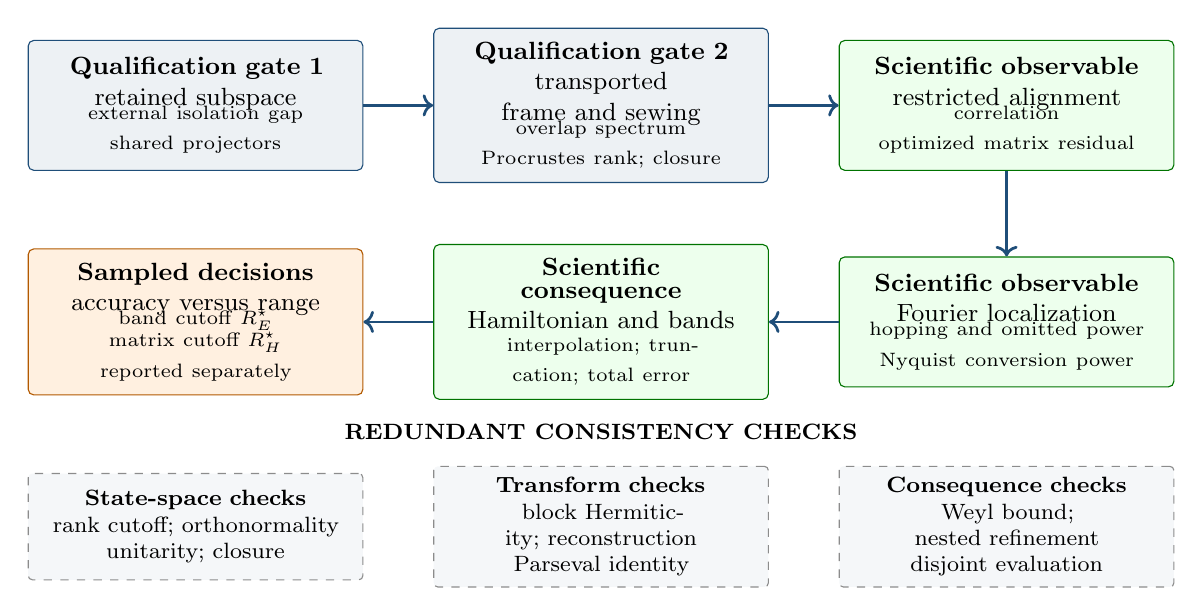
\begin{tikzpicture}[
  main/.style={rounded corners=2pt,minimum width=4.25cm,minimum height=1.65cm,
               text width=3.85cm,align=center,font=\small,inner sep=5pt},
  gate/.style={main,draw=protocolblue,fill=protocolblue!8},
  observable/.style={main,draw=green!45!black,fill=green!7},
  decision/.style={main,draw=orange!70!black,fill=orange!12},
  check/.style={rounded corners=1.5pt,minimum width=4.25cm,minimum height=1.35cm,
                text width=3.85cm,align=center,font=\footnotesize,
                draw=black!45,dashed,fill=protocolgray,inner sep=4pt},
  flow/.style={->,line width=1pt,protocolblue}
]
  \node[gate] (subspace) at (0,0) {
    \textbf{Qualification gate 1}\\
    retained subspace\\[-1mm]
    \scriptsize external isolation gap\\shared projectors
  };
  \node[gate] (frame) at (5.15,0) {
    \textbf{Qualification gate 2}\\
    transported frame and sewing\\[-1mm]
    \scriptsize overlap spectrum\\Procrustes rank; closure
  };
  \node[observable] (alignment) at (10.30,0) {
    \textbf{Scientific observable}\\
    restricted alignment\\[-1mm]
    \scriptsize correlation\\optimized matrix residual
  };
  \draw[flow] (subspace) -- (frame);
  \draw[flow] (frame) -- (alignment);

  \node[observable] (fourier) at (10.30,-2.75) {
    \textbf{Scientific observable}\\
    Fourier localization\\[-1mm]
    \scriptsize hopping and omitted power\\Nyquist conversion power
  };
  \node[observable] (consequence) at (5.15,-2.75) {
    \textbf{Scientific}\\[-1mm]
    \textbf{consequence}\\
    Hamiltonian and bands\\[-1mm]
    \scriptsize interpolation; truncation; total error
  };
  \node[decision] (range) at (0,-2.75) {
    \textbf{Sampled decisions}\\
    accuracy versus range\\[-1mm]
    \scriptsize band cutoff $R_E^\star$\\matrix cutoff $R_H^\star$\\reported separately
  };
  \draw[flow] (alignment) -- (fourier);
  \draw[flow] (fourier) -- (consequence);
  \draw[flow] (consequence) -- (range);

  \node[font=\footnotesize\bfseries] at (5.15,-4.15) {
    REDUNDANT CONSISTENCY CHECKS
  };
  \node[check] (statecheck) at (0,-5.35) {
    \textbf{State-space checks}\\
    rank cutoff; orthonormality\\unitarity; closure
  };
  \node[check] (transformcheck) at (5.15,-5.35) {
    \textbf{Transform checks}\\
    block Hermiticity; reconstruction\\Parseval identity
  };
  \node[check] (decisioncheck) at (10.30,-5.35) {
    \textbf{Consequence checks}\\
    Weyl bound; nested refinement\\disjoint evaluation
  };

\end{tikzpicture}
\caption{Diagnostic workflow. Blue boxes are qualification gates that must pass before
scientific interpretation. Green boxes are distinct observables or consequences; no
single scalar combines them. The orange box contains sampled range decisions made only
after the preceding fields are qualified. Dashed gray boxes collect redundant numerical
checks: they test the calculation but do not become additional observables or a second
scientific sequence.}
\label{fig:diagnostic-workflow}
\end{figure*}

The solid path in Fig.~\ref{fig:diagnostic-workflow} separates representation questions
from spectral ones. Restricted alignment asks what one global real rotation and one
positive scale cannot reproduce. Fourier diagnostics then measure where matrix power is
placed in real space. Only after explicit truncation are reconstructed-Hamiltonian and
band errors evaluated. Omitted block power is therefore a locality observable, not a
surrogate spectral-error bound.

The dashed boxes collect checks whose expected relationships are known independently.
Frame orthonormality and unitarity check transport; reconstruction and Parseval check the
finite transform; Weyl bounds, nested refinement, and the disjoint mesh check the
reported consequences and decisions. Closure eigenphases remain supporting sewing
diagnostics rather than convergence observables or topological claims.

For rank-two fields, reconstructed-Hamiltonian errors use
$\|\Delta H\|_F/(\sqrt{2}E_{\mathrm{ref}})$, whereas band errors use energy divided by $E_{\mathrm{ref}}$.
Weyl's inequality provides a one-way consistency bound between them, not an equality.
The same numerical tolerance applied to the two normalizations therefore defines two
separately named sampled cutoff questions; neither cutoff is silently substituted for
the other. Closure eigenphases are retained as sewing diagnostics, not as convergence
observables or topological claims. Detailed definitions are given in
Eqs.~\eqref{eq:truncation-hamiltonian-errors}--\eqref{eq:truncation-parseval-check}, and
all plotted diagnostic values are derived from the calculation tables.

\subsection{Resolution, verification, and control status}

Construction uses the nested momentum ladder
\begin{align}
 N&\in\{32,64,128,256,512\},\nonumber\\
 q_i&=-\frac12+\frac{i}{N},
 \qquad i=0,\ldots,N-1.
 \label{eq:construction-meshes}
\end{align}
The flat-parent study uses the same 65 amplitudes at every momentum resolution and
requires every implemented finite-mesh channel to pass on two successive refinements;
the continuous threshold laws are evaluated analytically rather than interpolated from
those nodes. The non-flat study applies the same momentum-refinement principle to parent,
frame, alignment, Fourier, and spectral channels. Neighbor-overlap singular values remain
rank-qualification gates rather than convergence observables. The reported `converged'
status concerns momentum refinement; non-flat results remain pointwise because no
continuous-amplitude reconstruction is claimed.

For the selected construction size $N_*$, post-construction evaluation uses
\begin{equation}
 M=4N_*+1
 \label{eq:evaluation-size}
\end{equation}
and the staggered coordinates
\begin{equation}
 \widetilde q_\ell=-\frac12+
 \frac{\ell+1/(N_*+1)}{M},
 \qquad \ell=0,\ldots,M-1,
 \label{eq:evaluation-mesh}
\end{equation}
which are disjoint from the construction nodes. This mesh probes interpolation and
truncation behavior without refitting and supplies no statistical independence or
parent-model validation.

Independent verifiers reconstruct the flat and dispersive parent matrices, eigenspaces,
transported frames, harmonic maxima, alignment losses, Fourier blocks, Parseval
relations, and reported convergence decisions without calling the producing action.
Verification discrepancies remain channel resolved. The truncation calculation now uses
every integer cutoff $R_c=0,\ldots,16$; its independent verifier reconstructs the fields
and first-passing decisions, and the threshold-adjacent refinement repeats them at
$N=128,256,512$ with $M=4N+1$. These are development outputs. Protocol freeze, retained
schemas and run identity, exact source provenance, and confirmatory retained execution
remain open and are not authorized by this manuscript.

Supplementary Secs.~S2--S4 provide the complete refinement rules, disjoint-mesh
interpretation, software ownership, independent-reconstruction contract, failure policy,
and control-status inventory.

\section{Results}

\subsection{Flat-parent benchmark}
\label{sec:exploratory-analysis}

Supplementary Fig.~S4 summarizes the development calculation for the
normalized smooth flat-parent family. It is not a retained run or evidence package.

The reference and transformed models retain the same Bloch eigenvalues across the
Brillouin zone. Their largest calculated band discrepancy is
$2.22\times10^{-16}$ [Fig.~S4(d)], so the conventional band
structure does not distinguish the two representations. The representation-aware
thresholds nevertheless increase continuously with amplitude
[Fig.~S4(a)]. Equations~\eqref{eq:minimum-operator-threshold}
and \eqref{eq:exact-spectrum-threshold-continuum} give normalized minimum-operator and
exact-spectrum joint thresholds of $0.8815978972$ and $1.0276174232$, respectively, at
$a=\pi/4$. Their separation shows that exact band agreement does not remove the
operator-level cost of identifying the representations.

The same mismatch appears in real-space locality. At $a=0$, all normalized hopping
weight outside the onsite block is below $1.3\times10^{-28}$ on the $N=512$ transform.
The total non-onsite weight rises to $0.2747231$ at $a=\pi/8$ and $0.7772149$ at
$a=\pi/4$. The cumulative tails in Fig.~S4(c) decay rapidly
with retained range, but their amplitude dependence is pronounced: the weight outside
$|R|\le4$ is $1.16\times10^{-8}$ at $a=\pi/8$ and $1.03\times10^{-5}$ at $a=\pi/4$.
The range-resolved map in Fig.~S4(e) confirms that the support
broadens continuously even though the bands remain unchanged. This is the calculated
counterpart of the exact flat-parent identity in
Eq.~\eqref{eq:continuum-three-way-identity}.

The numerical study separates momentum resolution from amplitude evaluation. For the
implemented flat-parent channels, refinement from $N=32$ through $N=512$ changes every
monitored momentum-dependent quantity only at approximately binary64 roundoff. The
continuous amplitude dependence does not rely on a uniform-grid interpolant:
Fig.~S4(a,b) evaluates the exact $J_0(2a)$ correlation and threshold laws directly. The
previous $N_a\le64$ midpoint test is retained only as a rejected interpolation
diagnostic, not as an unresolved control or a basis for the continuum claim. Numerical
hopping quantities remain values at their explicitly evaluated amplitudes.

This benchmark establishes the analytic mechanism and tests the flat-parent correlation,
threshold, band-discrepancy, and Fourier-locality channels. It does not test the frame,
admissible-set, witness, or separation-certificate workflow and does not establish
material realism. The parent is deliberately flat, and the reported hopping blocks are
finite-mesh Fourier coefficients. Final publication evidence requires a frozen retained
run and the additional controls stated below.

\subsection{Dispersive four-state benchmark}
\label{sec:nonflat-exploratory}

The typed dispersive implementation constructs the parent in
Eq.~\eqref{eq:parent-bloch}, selects the lower two-state spectral subspace, closes the
parallel-transport frame, and applies Eq.~\eqref{eq:attacked-matrix}.
Supplementary Fig.~S5 reports the resulting development diagnostics.
Momentum refinement is converged. Amplitude-dependent numerical statements are
pointwise at directly evaluated nodes; no between-node interpolation claim is made. The
result is not retained evidence.

At $N=512$, the minimum sampled external isolation gap is $1.0566461$, the minimum neighboring-frame
transport singular value is $0.9999997323$, and the largest independently reconstructed
result discrepancy is $3.09\times10^{-15}$. The largest computed band discrepancy over 65
amplitudes is $1.45\times10^{-15}$. At $a=\pi/4$, the discrete maximum correlation is
$0.5079908088$, the minimum operator threshold is $0.4004394264$, and the exact-spectrum
joint threshold is $0.4611609032$ [Fig.~S5(a)]. The comparison
non-onsite hopping weight increases from the reference value $0.0323839143$ to
$0.1761532501$. Its weight outside $|R|\le4$ is $8.43\times10^{-6}$, whereas the
reference value is $1.52\times10^{-18}$ [Fig.~S5(d)]. The full
amplitude-dependent redistribution is shown in
Figs.~S5(b)--(c). These are
finite-mesh observations, not the flat-parent identity in
Eq.~\eqref{eq:continuum-three-way-identity}.

The momentum disposition is `converged'. Between $N=256$ and $N=512$, the largest
selected outcome-channel change is $1.08\times10^{-11}$ and the largest
parent-invariant change is $1.67\times10^{-16}$
[Fig.~S5(e)]. Neighboring-frame overlap remains a qualification
lower bound rather than a convergence observable; shared parent eigenvalues and retained
spectral projectors provide the invariant cross-mesh checks. At $N_a=64$, the
largest correlation midpoint discrepancy is $3.49\times10^{-5}$ and the largest
hopping-block-power midpoint discrepancy is $1.39\times10^{-5}$
[Fig.~S5(f)]. The failing amplitude control is not overridden by
momentum convergence, roundoff-level band agreement, or apparently stable selected
thresholds.

\subsubsection{Bounded parent-family robustness study}

To distinguish the representation orbit from dependence on one selected parent, define
\begin{equation}
 K_\rho(q)=T_0+\rho\left(e^{2\pi iq}T_{+1}+e^{-2\pi iq}T_{-1}\right),
 \qquad 0\leq\rho\leq1.
 \label{eq:parent-homotopy}
\end{equation}
Thus $\rho=0$ is the onsite four-state parent and $\rho=1$ is the full parent in
Eq.~\eqref{eq:parent-bloch}. The onsite matrices, retained rank, frame protocol, and
rotation family are unchanged. Every sampled $\rho$ must independently clear the gap,
transport-rank, reconstruction, and momentum-refinement controls.

\begin{figure*}[t]
  \centering
  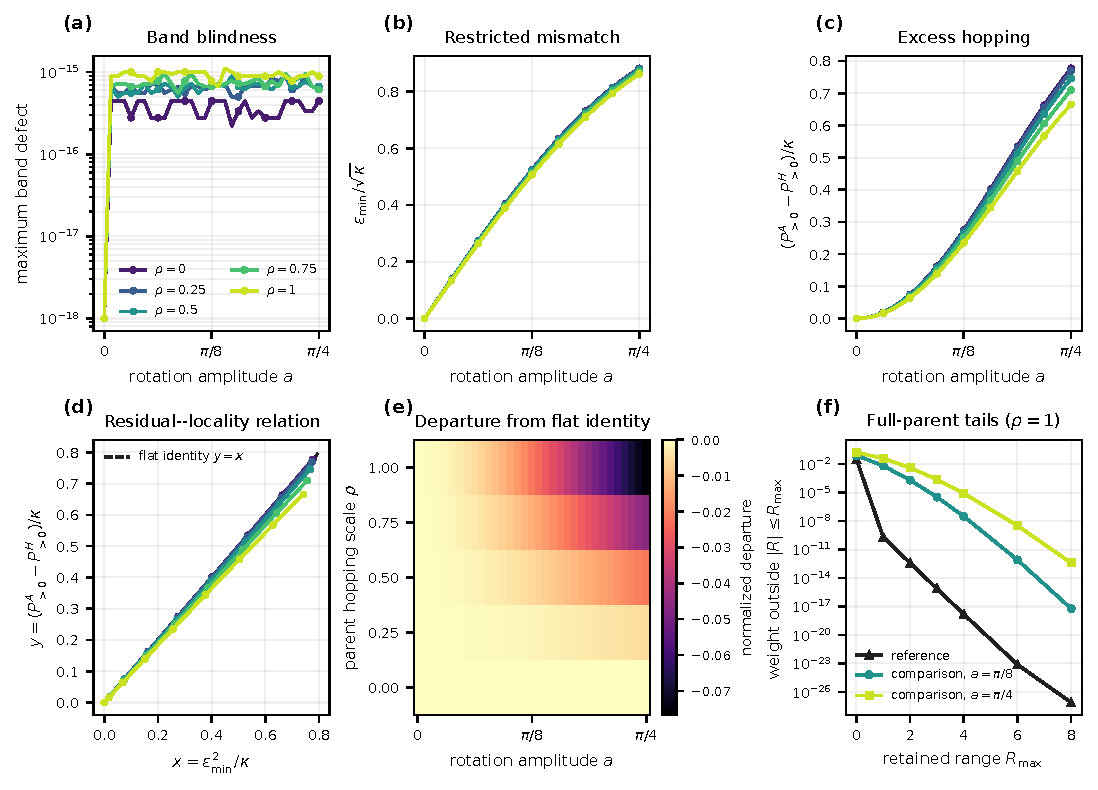
\includegraphics[width=\textwidth]
    {../../../../../experiments/model-adequacy/periodic1d/band-equivalence-versus-hopping-locality/analysis/band-equivalence-locality-scientific-story.pdf}
  \caption{Band equivalence and locality across the sampled parent family.
  \textbf{(a)} Maximum ordered-eigenvalue discrepancy; exact zeros are displayed at
  $10^{-18}$ on the logarithmic axis. \textbf{(b)} Minimum restricted-alignment
  threshold normalized by $\sqrt{\kappa}$; the dashed curve is the analytic flat-parent
  comparator. \textbf{(c)} Comparison-minus-reference non-onsite weight normalized by
  $\kappa$, with the flat analytic identity shown dashed. \textbf{(d)} Parametric
  relation between normalized squared operator residual $x$ and normalized excess
  locality weight $y$; the dashed diagonal is the flat identity $y=x$.
  \textbf{(e)} Directly calculated departure $y-x$ over the $5\times33$ sampled
  parameter pairs. \textbf{(f)} Full-parent cumulative tails at selected amplitudes.
  Colors identify the parent hopping scales in panel (a), markers show every fourth
  amplitude sample, and connecting lines are guides to the eye. All five momentum
  studies through $N=256$ are `converged'; the finite $\rho$ and amplitude inventories
  are not continuous-domain certificates. This is development analysis, not a retained
  evidence run or material validation.}
  \label{fig:parent-family-analysis}
\end{figure*}

\subsubsection{Implemented metrics and interpretation of the parent-family figure}

The implemented calculation concerns complete finite-mesh retained Hamiltonians, not
range-truncated approximations. For each sampled parent scale $\rho$, the four-state
parent is diagonalized, the lower two-dimensional spectral subspace is transported into
a periodic orthonormal frame, and the resulting $2\times2$ retained field $H_\rho(q_i)$
is formed. The comparison field is
\begin{align}
 A_{\rho,a}(q_i)&=U_a(q_i)^\dagger H_\rho(q_i)U_a(q_i),\nonumber\\
 U_a(q)&=R(a\sin 2\pi q).
 \label{eq:implemented-parent-family-comparison}
\end{align}
Equation~\eqref{eq:implemented-parent-family-comparison} is a pointwise unitary change of
representation. The complete reference and comparison fields therefore have identical
ordered eigenvalues in exact arithmetic. The reported band discrepancy is
\begin{equation}
 \Delta_{\mathrm{band}}(\rho,a)=
 \max_{i,n}\frac{|\varepsilon_n[A_{\rho,a}(q_i)]
                       -\varepsilon_n[H_\rho(q_i)]|}{E_{\mathrm{ref}}}.
 \label{eq:implemented-band-discrepancy}
\end{equation}
It is a numerical confirmation of the constructed similarity relation, not evidence that
two independently derived material Hamiltonians agree. Exact zeros in
Fig.~\ref{fig:parent-family-analysis}(a) are placed at $10^{-18}$ only for logarithmic
display.

Let $H_\rho^\circ(q_i)$ denote the traceless retained field and define
\begin{equation}
 \kappa_\rho=\frac{1}{N}\sum_i
 \frac{\|H_\rho^\circ(q_i)\|_F^2}{2E_{\mathrm{ref}}^2}.
 \label{eq:implemented-splitting-scale}
\end{equation}
Continuous harmonic maximization gives the largest normalized correlation
$\mu_{\rho,a,\max}$ attainable by one momentum-independent real rotation. Because the
candidate also admits one positive splitting multiplier, its irreducible matrix-loss
threshold is
\begin{equation}
 \epsilon_{\min}(\rho,a)
 =\sqrt{\kappa_\rho\left[1-\max(0,\mu_{\rho,a,\max})^2\right]}.
 \label{eq:implemented-minimum-threshold}
\end{equation}
Consequently, panel (b) plots $\epsilon_{\min}/\sqrt{\kappa_\rho}$ and panel (d) uses
\begin{equation}
 x=\frac{\epsilon_{\min}^2}{\kappa_\rho}.
 \label{eq:implemented-normalized-residual}
\end{equation}
This metric answers a restricted representation question: how much of the
momentum-dependent comparison field cannot be reproduced by one global real rotation,
one positive scale, and the common mean-energy field. It is not a distance between
abstract operators under arbitrary momentum-dependent unitary equivalence.

For centered finite-mesh cell displacements, the implementation constructs Fourier
blocks $T_R^{H_\rho}$ and $T_R^{A_{\rho,a}}$. In the Wannier representation generated
by the chosen periodic Bloch frame, their entries have the tight-binding meaning
\begin{equation}
 [T_R^X]_{mn}=\langle 0m|\widehat X|Rn\rangle,
 \qquad
 X_{mn}(q)=\sum_R e^{2\pi iqR}[T_R^X]_{mn},
 \label{eq:implemented-wannier-hopping}
\end{equation}
where $|Rn\rangle$ is the Wannier orbital in cell $R$ associated with retained orbital
$n$. On the finite construction mesh this is a discrete, potentially aliased Wannier
representation rather than a continuous localization certificate. A momentum-dependent
Bloch-frame rotation mixes Wannier orbitals across lattice cells and therefore
redistributes the real-space matrix elements in
Eq.~\eqref{eq:implemented-wannier-hopping} without changing the complete Bloch spectrum.
The implementation assigns each block the per-retained-state power
\begin{equation}
 p_R^X=\frac{\|T_R^X\|_F^2}{2E_{\mathrm{ref}}^2},
 \qquad
 P_{>0}^X=\sum_{R\ne0}p_R^X,
 \qquad X\in\{H_\rho,A_{\rho,a}\}.
 \label{eq:implemented-hopping-power}
\end{equation}
Panel (c) plots the signed excess
\begin{equation}
 y=\frac{P_{>0}^{A_{\rho,a}}-P_{>0}^{H_\rho}}{\kappa_\rho}.
 \label{eq:implemented-normalized-excess}
\end{equation}
Equivalently,
\begin{equation}
 p_R^X=\frac{1}{2E_{\mathrm{ref}}^2}\sum_{m,n}
 |\langle 0m|\widehat X|Rn\rangle|^2.
 \label{eq:implemented-hopping-power-matrix-elements}
\end{equation}
Thus $p_R^X$ is an entrywise squared-amplitude diagnostic for hopping between cell
Wannier orbitals, summed over all retained-orbital pairs and normalized per retained
state and by $E_{\mathrm{ref}}^2$. It is not a transition probability. Although both terms in the
numerator are nonnegative,
their difference is not a norm and need not be nonnegative for an arbitrary family. It
is positive for the sampled family.
At $\rho=0$, the reference has no non-onsite hopping and the flat-parent theorem gives
$y=x$. For $\rho>0$, the reference already contains non-onsite blocks. Writing
$T_R^{A}=T_R^{H}+\delta T_R$ shows that the excess contains both
$\|\delta T_R\|_F^2$ and the cross term
$2\operatorname{Re}\operatorname{tr}[(T_R^H)^\dagger\delta T_R]$. No theorem therefore
identifies $y$ with the restricted residual $x$ for a dispersive parent. Panels (d) and
(e) report the calculated relation and the diagnostic departure $y-x$ rather than
assuming the flat identity. The systematic negative departure means that the increase in
non-onsite block power accounts for less than the full normalized restricted residual in
this family; it is not a failure of band equivalence.

Finally, panel (f) reports
\begin{equation}
 P_{>R_c}^{X}=\sum_{|R|>R_c}p_R^X
 \label{eq:implemented-cumulative-tail}
\end{equation}
for the full parent $\rho=1$ at selected amplitudes. This is the hopping power omitted by
a symmetric range cutoff. The complete-model calculation underlying panel (f) does not
construct the truncated Hamiltonian; panel (f) measures representation-dependent
real-space compactness rather than spectral truncation error. The separate truncation
action below measures that spectral effect.

This result matters for reduced solid-state modeling because retained-subspace gauge
controls the cost of representing a complete Bloch field with real-space hopping
blocks. Panels (a)--(e) establish, on the declared sample nodes, that exact band
equivalence coexists with a large restricted representation residual and redistributed
hopping power throughout the parent homotopy. They do not establish physical
inequivalence of the complete gauge-related Hamiltonians. The homotopy is synthetic, the
five $\rho$ values and 33 amplitudes are direct samples, and the coefficients are
finite-mesh Fourier coefficients rather than a continuous-domain or
material-localization certificate.

All five momentum studies return `converged'. The smallest sampled external isolation gap decreases
from $1.3436583E_{\mathrm{ref}}$ at $\rho=0$ to $1.0566461E_{\mathrm{ref}}$ at $\rho=1$, while the reference
non-onsite weight rises from numerical noise to $0.0323839$. At $a=\pi/4$, the
scale-normalized minimum threshold changes from $0.8815979$ to $0.8613625$, and the
excess comparison non-onsite weight changes from $0.1431824$ to $0.1437693$
[Fig.~\ref{fig:parent-family-analysis}(b)--(c)]. The normalized flat-identity departure
$y-x$ changes from roundoff at $\rho=0$ to $-0.0767265$ at $\rho=1$
[Fig.~\ref{fig:parent-family-analysis}(d)--(e)]. Thus the restricted mismatch and excess
hopping remain large while the exact flat residual--tail identity deforms systematically
with parent dispersion. The representation-induced mismatch is therefore observed
throughout the sampled homotopy, not only for the endpoint parent.
The five $\rho$ values and 33 amplitudes remain finite samples; they do not establish a
continuous-$\rho$ bound or resolve amplitude interpolation.

\subsubsection{Finite-range band consequences}

The consequence action uses $N=256$ and a disjoint evaluation mesh with $M=1025$. It
also uses the same five parent scales, 33 pointwise amplitudes, and cutoffs
$R_c\in\{0,1,2,3,4,6,8,12,16,24,32,48,64\}$. These are development samples rather than
a frozen retained inventory. The minimum periodic construction--evaluation mesh
separation is $1.48\times10^{-8}$.

Across the sampled family, direct pointwise unitary comparison preserves the two bands
within $1.33\times10^{-15}E_{\mathrm{ref}}$, and the maximum full-comparison interpolation discrepancy on
the disjoint mesh is $2.40\times10^{-14}E_{\mathrm{ref}}$. At $(\rho,a)=(1,\pi/4)$, $R_c=3$ gives a
reference maximum band error of $5.53\times10^{-8}E_{\mathrm{ref}}$ but a comparison total band error
of $1.86\times10^{-2}E_{\mathrm{ref}}$. At $R_c=8$, those values are
$4.22\times10^{-14}E_{\mathrm{ref}}$ and $8.65\times10^{-7}E_{\mathrm{ref}}$, respectively
[Fig.~S6(a)]. The same ordering persists
through the five sampled parent scales [Fig.~S6(b)]. At
the sampled nodes, complete band-equivalent Hamiltonians therefore require substantially
different finite hopping ranges for comparable band accuracy.

Supplementary Fig.~S6(c) shows close tracking between square-root
omitted power and maximum band error in this synthetic inventory. The protocol infers no
equality, upper bound, or universal range-to-accuracy law from that correlation. The
action excludes velocity, curvature, and physical effective mass. Cutoff targets and the
final cap remain unfrozen. Independent development reconstruction and strict truncation
serialization are implemented; a retained-evidence
contract and authorized retained execution are not.

To express this difference as an accuracy-versus-cost diagnostic, let
$\mathcal R_{\mathrm{samp}}$ denote the declared cutoff inventory and define the first
sampled passing cutoff
\begin{equation}
 \widehat R_c^\star(\rho,a;\tau)
 =\min_{R_c\in\mathcal R_{\mathrm{samp}}}
 \left\{R_c:\epsilon_{\max}(\rho,a,R_c)\le\tau E_{\mathrm{ref}}\right\}.
 \label{eq:first-sampled-passing-cutoff}
\end{equation}
The hat records the sampled $(\rho,a)$ domain and finite declared cap; every integer
cutoff within $R_c=0,\ldots,16$ is included. The sampled representation-induced range inflation is
\begin{equation}
 \Delta\widehat R_c^\star
 =\widehat R_{c,\mathrm{comparison}}^\star
  -\widehat R_{c,\mathrm{reference}}^\star.
 \label{eq:sampled-range-inflation}
\end{equation}
For the reference, $\epsilon_{\max}$ is the maximum band error after ordinary-lattice
truncation. For the comparison, it is the total spectral error relative to the direct
comparison field, so the requested cutoff includes its separately reported
finite-interpolant discrepancy.

\begin{figure*}[t]
  \centering
  \includegraphics[width=0.96\textwidth]
    {../../../../../experiments/model-adequacy/periodic1d/band-equivalence-versus-hopping-locality/analysis/range-inflation-preview.pdf}
  \caption{Exploratory sampled range inflation at four band-error targets. Each tile is
  one directly sampled $(\rho,a)$ pair, and color gives
  $\Delta\widehat R_c^\star$ from Eq.~\eqref{eq:sampled-range-inflation}. No smoothing
  or continuous interpolation is applied. At the dispersive endpoint
  $(\rho,a)=(1,\pi/4)$, the sampled additional ranges are $5$, $6$, $6$, and $7$ for
  targets $10^{-6}$, $10^{-8}$, $10^{-10}$, and $10^{-12}$, respectively. Stair-step
  boundaries reflect the integer-valued decision rule and sampled parameter grid; they
  are not caused by skipped cutoffs and are not physical discontinuities.}
  \label{fig:range-inflation-preview}
\end{figure*}

Positive sampled range inflation occurs at 159 of 165 sampled $(\rho,a)$ points for the
$10^{-6}$ and $10^{-8}$ targets and at 156 points for both $10^{-10}$ and $10^{-12}$.
At $(\rho,a)=(1,\pi/4)$, the first sampled passing cutoffs are respectively $(3,8)$,
$(4,10)$, $(6,12)$, and $(7,14)$ for the reference and comparison. In one dimension, a
symmetric cutoff retains $2R_c+1$ displacement blocks, so the $10^{-8}$ example
corresponds to 9 versus 21 possible block positions before any additional zero-block
compression. This is an operational measure of representation
cost, not physical inequivalence: the complete models remain pointwise unitarily
related before truncation.

Complete-band agreement does not certify an economical finite-range model. Equal cutoff
is not a representation-neutral comparison; equal declared accuracy is. This controlled
calculation supplies a benchmark for that comparison and attributes the observed error
to conversion, interpolation, or deliberate truncation. Material-derived Wannier
Hamiltonians and higher dimensions remain outside the demonstrated scope; in higher
dimensions, the retained-neighbor count generally grows more rapidly with range. The dense inventory removes skipped-integer ambiguity. Independent reconstruction gives
a maximum absolute discrepancy of $4.61\times10^{-13}$, and threshold-adjacent checks
show no first-passing decision changes from $N=128$ through 512. Protocol freeze, exact
source provenance, retained execution, and retained-package verification are still
required before Fig.~\ref{fig:range-inflation-preview} can serve as retained evidence.

\paragraph{Error-channel accounting.}
Figure~\ref{fig:truncation-error-decomposition} separates the numerical error channels
that underlie the range comparison.

\begin{figure*}[t]
  \centering
  \includegraphics[width=\textwidth]
    {../../../../../experiments/model-adequacy/periodic1d/band-equivalence-versus-hopping-locality/analysis/truncation-error-channel-decomposition.pdf}
  \caption{The four approximation channels are reported separately.
  \textbf{(a)} Normalized Frobenius power in the centered cyclic Nyquist block removed
  during conversion to an ordinary-lattice inventory; this is conversion power, not an
  off-node spectral error. The gray band spans the reference values across the five
  sampled parents. \textbf{(b)} Maximum spectral discrepancy of the untruncated finite
  interpolant relative to the directly evaluated comparison field on the disjoint mesh.
  \textbf{(c)} Maximum spectral change caused only by deliberate ordinary-lattice
  truncation at $a=\pi/4$. \textbf{(d)} Maximum total spectral error of each truncated
  model relative to the direct comparison field. The dashed line marks the $\rho=1$
  interpolation-discrepancy scale. Spectral norms are not stacked or treated as additive:
  their underlying matrix and eigenvalue errors reinforce or partially cancel. Lines
  connect sampled values as guides to the eye.}
  \label{fig:truncation-error-decomposition}
\end{figure*}

The centered-Nyquist conversion power remains between
$8.87\times10^{-32}E_{\mathrm{ref}}^2$ and $1.14\times10^{-31}E_{\mathrm{ref}}^2$ over the sampled family, while
the largest finite-interpolant spectral discrepancy is $2.35\times10^{-14}E_{\mathrm{ref}}$. At the
fully dispersive endpoint, the deliberate truncation error falls from
$5.25\times10^{-1}E_{\mathrm{ref}}$ at $R_c=0$ to $8.65\times10^{-7}E_{\mathrm{ref}}$ at $R_c=8$ and
$2.78\times10^{-11}E_{\mathrm{ref}}$ at $R_c=12$. By $R_c=16$, the total channel is
$4.69\times10^{-14}E_{\mathrm{ref}}$ and is controlled by interpolation and binary64-scale numerical
floors rather than the short-range truncation trend. Cyclic conversion, finite
interpolation, deliberate truncation, and total spectral consequence therefore remain
distinct.

\subsection{Diagnostic results}
\label{sec:diagnostic-results}

The diagnostic ledger supports the finite-range interpretation without replacing the
scientific observables. Across the five sampled parent scales, the minimum external isolation gap
remains at least $1.056646E_{\mathrm{ref}}$, the minimum transport singular value exceeds
$0.9999989$, and frame orthonormality, unitarity, periodic closure, Hermiticity,
reconstruction, and Parseval discrepancies remain near their declared numerical floors. The
largest off-node interpolation discrepancies are $2.46\times10^{-14}$ in the normalized
Hamiltonian channel and $2.35\times10^{-14}$ in the band channel, below the displayed
truncation scales.

Every sampled spectral error satisfies its Frobenius perturbation bound, but the ratio
to that bound ranges from approximately $0.0087$ to $0.9984$; band agreement therefore
does not uniformly imply matrix agreement. At the $10^{-8}$ target, Hamiltonian and
spectral criteria select the same comparison cutoff at 158 of 165 sampled $(\rho,a)$
points and give the same endpoint cutoff 10; the reference criteria agree at all 165
points and give endpoint cutoff 4. The two criteria remain separately
named. Supplementary Sec.~S5 and Figs.~S1--S3 report the complete frame-sewing,
Hamiltonian--spectral, and sampled-decision diagnostics.

\section{Discussion}

\subsection{Representation efficiency}

Theorem~\ref{thm:exact-loss-geometry} is not specific to the numerical parent matrices.
It applies to any sampled rank-two Hermitian field with positive weights, a comparison
target related by unitary conjugation, and the trace--traceless candidate family in
Eq.~\eqref{eq:candidate}. The parent, momentum dependence, and continuous global
alignment enter the optimized geometry through $\kappa$ and $\mu_{\max}$.

An instance-specific conclusion applies only to the stated parent model, retained
rank-two subspace, frame convention, comparison representation, candidate family,
parameter rectangle, continuous global real-rotation family, thresholds, numerical
resolution, and data roles. A compatible result establishes that one parameter pair
meets both declared limits in this controlled setting. A separated result establishes
that the admissible regions exceed the declared separation resolution under the verified
geometric premises. Neither result establishes material validity, parent-model
correctness, uncertainty quantification, uniqueness, continuum convergence, or adequacy
under unrestricted momentum-dependent unitaries.

The frame, matrix loss, and locality norms are basis dependent by design; the spectral
loss is basis invariant. Under the full generating $U_a(q)$, $H(q)$ and $A_a(q)$ are
unitarily equivalent representations and their abstract-operator residual is zero. The
reported nonzero residual answers the restricted question in which only one
momentum-independent real rotation identifies retained coordinates. This distinction is
the scientific question, not a technical inconvenience. Spectral convergence likewise
does not imply convergence of represented matrices, hopping blocks, or geometric
certificates, so every applicable channel is tested explicitly.

\subsection{Diagnostics}

The diagnostic ledger rules out three simple numerical explanations for the reported
range inflation on the sampled controls. First, the retained subspace remains separated
and the transport overlaps remain full rank. Second, unitary, closure, Hermiticity,
reconstruction, and Parseval checks remain near their declared numerical floors. Third,
the disjoint-mesh interpolation channel is far below the displayed truncation errors.
The range comparison is therefore not being set by an evident gap closure, frame-rank
failure, non-Hermitian evaluation, or interpolation floor.

The diagnostics do not supply a causal law connecting closure holonomy, restricted
alignment residual, hopping redistribution, and truncation error. Those quantities
answer different questions and are intentionally not collapsed into one score. In
particular, the closure phases vary smoothly with parent dispersion but are neither
acceptance thresholds nor topological claims. Omitted block power measures locality but
is not a universal spectral-error bound. The observed near-saturation of the Frobenius
bound at some cutoffs and its looseness at others explains why matrix and band accuracy
must both remain visible.

For the present headline, the first sampled passing cutoff remains the explicitly named
spectral decision used in Eq.~\eqref{eq:first-sampled-passing-cutoff}. The Hamiltonian
cutoff is a parallel diagnostic, not a retrospective change to that decision rule. A
future protocol may prescribe separate spectral and Hamiltonian accuracy targets, but it
should not replace them with a single combined score.

\subsection{Limitations and scope}

No Quantum ESPRESSO or Wannier90 calculation occurs in this controlled protocol. A
separate retained single-band Fourier-reduction run verifies an earlier scalar synthetic
reduction chain; Supplemental Sec.~S7 reports it as a precursor with an independent
experiment identity. Its retained status does not make it evidence for the present
rank-two range-inflation claim. A material application requires separate authorization
and a design fixing the structure, pseudopotentials, exchange--correlation approximation,
cutoffs, meshes, Wannier windows and projections, energy alignment, resource estimates,
and provenance.

\subsection{Architectural roadmap and controlled validation ladder}
\label{sec:validation-ladder}

The synthetic, fully known four-state parent is the transparent starting point of a
controlled validation program, not a proxy material. In a material-derived workflow,
disentanglement windows, projections, reciprocal meshes, gauge construction, energy
alignment, and finite-range truncation can all affect the resulting representation.
Beginning with a hidden target would make representation-induced locality difficult to
distinguish from parent-model, discretization, and model-reduction errors.

The planned program therefore expands along two separately controlled directions, as
shown in Fig.~\ref{fig:validation-ladder}. The spatial direction proceeds from the
present one-dimensional chain to independent two- and three-dimensional benchmarks,
then to anisotropic support and general non-orthogonal lattices. At each of these stages
the generating operator remains known, so lattice metrics, frame transport, reciprocal
sewing, Fourier reconstruction, support conventions, and range decisions can be checked
against ground truth.

\begin{figure*}[t]
\centering
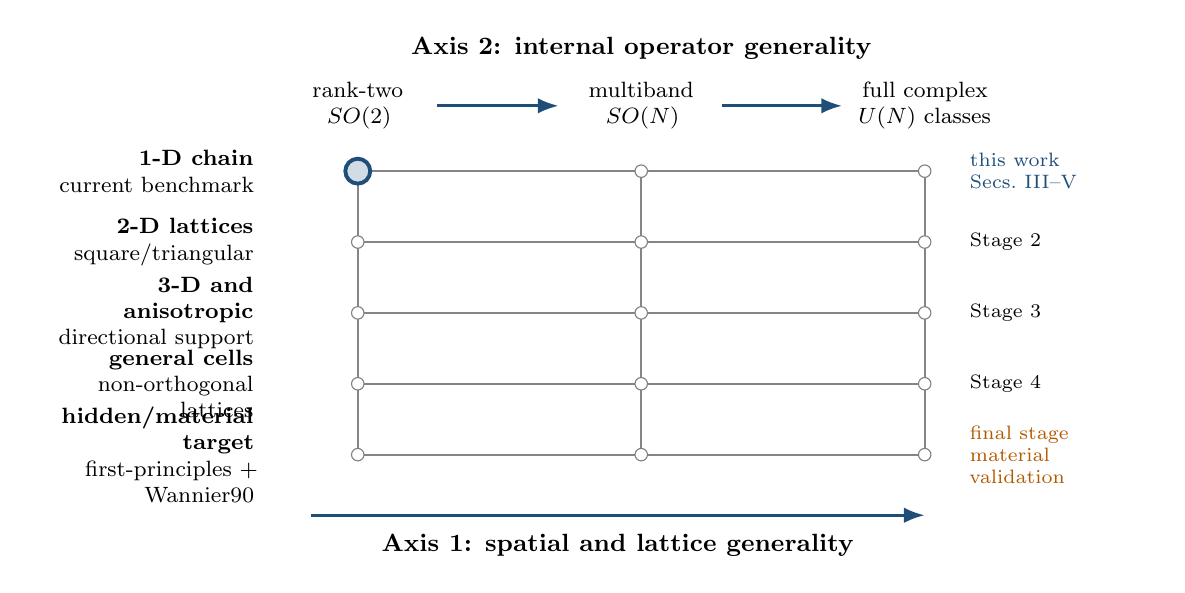
\begin{tikzpicture}[
  >=Latex,
  gridline/.style={line width=0.75pt,black!48},
  progression/.style={->,line width=1pt,protocolblue},
  stage/.style={font=\footnotesize,align=flush right,text width=2.75cm},
  column/.style={font=\footnotesize,align=flush center,text width=3.1cm},
  note/.style={font=\scriptsize,align=flush left,text width=2.25cm},
  point/.style={circle,draw=black!50,fill=white,minimum size=4.5pt,inner sep=0pt},
  current/.style={circle,draw=protocolblue,line width=1.4pt,fill=protocolblue!20,
                  minimum size=9pt,inner sep=0pt}
]
  % Internal-operator axis and column labels.
  \node[font=\small\bfseries,anchor=south] at (4.15,4.95)
    {Axis 2: internal operator generality};
  \node[column] at (0.55,4.48) {rank-two\\$SO(2)$};
  \node[column] at (4.15,4.48) {multiband\\$SO(N)$};
  \node[column] at (7.75,4.48) {full complex\\$U(N)$ classes};
  \draw[progression] (1.55,4.48) -- (3.10,4.48);
  \draw[progression] (5.18,4.48) -- (6.70,4.48);

  % Spatial/lattice rows.
  \node[stage] at (-2.15,3.65) {\textbf{1-D chain}\\current benchmark};
  \node[stage] at (-2.15,2.75) {\textbf{2-D lattices}\\square/triangular};
  \node[stage] at (-2.15,1.85) {\textbf{3-D and anisotropic}\\directional support};
  \node[stage] at (-2.15,0.95) {\textbf{general cells}\\non-orthogonal lattices};
  \node[stage] at (-2.15,0.05) {\textbf{hidden/material target}\\first-principles + Wannier90};

  % Full two-axis ladder.
  \foreach \y in {0.05,0.95,1.85,2.75,3.65}
    \draw[gridline] (0.55,\y) -- (7.75,\y);
  \foreach \x in {0.55,4.15,7.75}
    \draw[gridline] (\x,0.05) -- (\x,3.65);
  \foreach \x in {0.55,4.15,7.75}
    \foreach \y in {0.05,0.95,1.85,2.75,3.65}
      \node[point] at (\x,\y) {};
  \node[current] at (0.55,3.65) {};

  % Stage annotations.
  \node[note,protocolblue] at (9.45,3.65)
    {this work\\Secs.~III--V};
  \node[note] at (9.45,2.75) {Stage 2};
  \node[note] at (9.45,1.85) {Stage 3};
  \node[note] at (9.45,0.95) {Stage 4};
  \node[note,orange!70!black] at (9.45,0.05)
    {final stage\\material validation};

  \draw[progression] (-0.05,-0.72) -- (7.75,-0.72);
  \node[font=\small\bfseries,anchor=north] at (3.85,-0.83)
    {Axis 1: spatial and lattice generality};
\end{tikzpicture}
\caption{Two-axis controlled validation ladder. Along Axis~1, the known-parent stages
introduce spatial and structural degrees of freedom while retaining exact access to the
generating operator $\widehat K(q)$; the final hidden/material row deliberately removes
that access. Axis~2 expands the internal comparison spaces from global rank-two $SO(2)$
rotations to multiband $SO(N)$ and complex $U(N)$ classes. This work establishes the
ground-truth benchmark at the blue origin (1-D, rank-two $SO(2)$). Every other grid point
is a prospective validation stage rather than a result of this paper.}
\label{fig:validation-ladder}
\end{figure*}

The internal direction is distinct from dimensional extension. It proceeds from the
present rank-two real gauge and one global $SO(2)$ comparison fit to controlled
higher-rank real classes and then to complex, non-Abelian $U(N)$ gauge classes. At every
rung, the momentum-dependent generating transformation and the more restricted
identification allowed during comparison must be stated separately. Consequently,
higher dimension alone does not answer the multiband-gauge question, and higher rank
alone does not qualify lattice range conventions.

The two directions meet only after their diagnostics have been exercised on known
operators. Hidden-target effective Hamiltonians and material-derived Wannier
Hamiltonians are then a final validation setting, where the framework must separate
parent-model, discretization, model-reduction, and deliberate truncation errors rather
than attributing all disagreement to gauge choice. The present theorems supply exact
rank-two anchors for that program; they do not assert that the same closed forms hold on
higher-rank manifolds.

\clearpage
\section{Conclusions}

Band equivalence does not determine hopping locality. For the rank-two candidate family,
spectral and restricted-alignment losses share an exact quadratic curvature, and the
smooth rotation continuum converts that geometry into analytic acceptance thresholds.
For a flat traceless parent, the squared irreducible matrix residual equals the induced
non-onsite Fourier weight. The dispersive parent homotopy preserves the same qualitative
separation while deforming the flat identity in a controlled manner.

The finite-range calculation supplies the practical consequence. At fixed sampled band
accuracy, gauge-related complete Hamiltonians require different hopping cutoffs after
truncation. This result concerns representation efficiency rather than physical
inequivalence: the complete fields remain pointwise unitarily related. Explicit
separation of cyclic conversion, interpolation, deliberate truncation, and total
spectral error prevents the range comparison from absorbing unrelated numerical effects.

The diagnostic results support that interpretation without becoming a separate physical
claim. The sampled subspaces remain isolated, transport and reciprocal sewing remain
well conditioned, redundant Fourier and matrix identities close at numerical precision,
and interpolation remains below the reported truncation scales. Hamiltonian and spectral
errors usually select the same sampled ranges but expose isolated cases in which band
agreement hides matrix disagreement; they must therefore remain separately visible.

The analytic statements are complete within their declared rank-two and alignment
assumptions. The numerical range-inflation map remains a sampled development result.
Its dense integer cutoffs, threshold-adjacent resolution checks, and independent
first-passing reconstruction are complete for the declared development grid. Protocol
freeze, exact source provenance, retained execution, and retained-package verification
are still required before it becomes final retained publication evidence. Higher-dimensional
rank-two benchmarks~\cite{Ragasa2026b} and higher-rank multiband controls~\cite{Ragasa2026c}
form the next controlled rungs; a first-principles bulk-silicon reduction~\cite{Ragasa2026d}
is the planned material endpoint rather than an omitted preliminary case.

\section*{Acknowledgments}
\emph{Author to complete before submission.}

\section*{Data and code availability}
The project repository maintains the publication-independent experiment, analyses,
figure sources, and software contracts in its periodic one-dimensional
band-equivalence/locality experiment directory. The present numerical figures are
development artifacts rather than a retained production package. A public archival
identifier, exact source revision, and authorized release record must be supplied before
submission.

\bibliographystyle{unsrt}
\bibliography{references,../../unpublished-papers}

\end{document}
